\documentclass{article}
% \usepackage{neurips_2023}
\usepackage[preprint]{neurips_2023}
\usepackage[utf8]{inputenc}
\usepackage{amsfonts}
\usepackage[mathscr]{euscript}
\usepackage[numbers]{natbib} % has a nice set of citation styles and commands
\usepackage{mathtools} % amsmath with fixes and additions
\usepackage{bbm}
% \usepackage{siunitx} % for proper typesetting of numbers and units
\usepackage{booktabs} % commands to create good-looking tables
\usepackage{tikz} % nice language for creating drawings and diagrams
% \usepackage{algorithm2e}
\usepackage{boxedminipage}
\usepackage{alltt}
\usepackage{bm}
\usepackage{geometry}
\usepackage{hyperref}
\usepackage{authblk}
\usepackage{lineno}         % Enables line numbers
\usepackage{lipsum}
\geometry{
% a4paper,
 total={150mm,200mm},
 left=30mm,right = 30mm,
 top=30mm,bottom =30mm,
}

\usepackage{graphicx}

% \linenumbers

\DeclareMathOperator{\defeq}{\stackrel{\text{def}}{=}}
\DeclareMathOperator{\assumedeq}{\stackrel{\text{assumed}}{=}}
\DeclareMathOperator{\Tr}{\text{Tr}}
\DeclarePairedDelimiter{\nint}\lfloor\rceil

% Emergent Abilities Don't Exist
% 
\title{Are Emergent Abilities of Large Language Models a Mirage?}
\author[]{Rylan Schaeffer}
\author[]{Brando Miranda}
\author[]{Sanmi Koyejo}

\affil[]{Computer Science, Stanford University}


% \date{Winter 2023}

\begin{document}

\maketitle

% 2023/05/16 Abstract
% Recent work claims that large language models display \textit{emergent abilities}, abilities not present in smaller-scale models that are present in larger-scale models. What makes emergent abilities intriguing is two-fold: their \textit{sharpness}, transitioning seemingly instantaneously from not present to present, and their \textit{unpredictability}, appearing at seemingly unforeseeable model scales.
%     Here, we present an alternative explanation for emergent abilities: that for a particular task and model family, when analyzing fixed model outputs, one can choose a metric which leads to the inference of an emergent ability or another metric which does not.
%     Thus, our alternative suggests that existing claims of emergent abilities are creations of the researcher's analyses, not fundamental changes in model behavior on specific tasks with scale.
%     We present our explanation in a simple mathematical model, then test it in three complementary ways: we (1) make, test and confirm three predictions on the effect of metric choice using the InstructGPT/GPT-3 family on tasks with claimed emergent abilities, (2) make, test and confirm two predictions about metric choices in a meta-analysis of emergent abilities on BIG-Bench; and (3) show how similar metric decisions suggest apparent emergent abilities on vision tasks in diverse deep network architectures (convolutional, autoencoder, transformers).
%     In all three analyses, we find strong supporting evidence that emergent abilities may not be a fundamental property of scaling AI models.

\begin{abstract}
Recent work claims that large language models display \textit{emergent abilities}, abilities not present in smaller-scale models that are present in larger-scale models.
What makes emergent abilities intriguing is two-fold: their \textit{sharpness}, transitioning seemingly instantaneously from not present to present, and their \textit{unpredictability}, appearing at seemingly unforeseeable model scales.
Here, we present an alternative explanation for emergent abilities: that for a particular task and model family, when analyzing fixed model outputs, emergent abilities appear due the researcher’s choice of metric rather than due to fundamental changes in model behavior with scale. Specifically, nonlinear or discontinuous metrics produce apparent emergent abilities, whereas linear or continuous metrics produce smooth, continuous, predictable changes in model performance.
We present our alternative explanation in a simple mathematical model, then test it in three complementary ways: we (1) make, test and confirm three predictions on the effect of metric choice using the InstructGPT/GPT-3 family on tasks with claimed emergent abilities, (2) make, test and confirm two predictions about metric choices in a meta-analysis of emergent abilities on BIG-Bench; and (3) show how to choose metrics to produce never-before-seen seemingly emergent abilities in multiple vision tasks across diverse deep networks.
Via all three analyses, we provide evidence that alleged emergent abilities evaporate with different metrics or with better statistics, and may not be a fundamental property of scaling AI models.
\end{abstract}

%---------------------------------
\section{Introduction}
\label{sec:intro}
%---------------------------------


The popularity of powerful diffusion models has led to remarkable progress in the field of content generation. For instance, text-to-image (T2I) models are capable of generating diverse and vivid images from text prompts, encompassing various visual concepts. This great success can be attributed not only to the advancement of models but also to the availability of various image data over the Internet.
Constrastingly, text-to-video (T2V) models fall short of the data categories especially in styles, since existing videos predominantly feature photorealism. While these strategies, like initializing weights from well-trained T2I models or joint training with image and video datasets, can help mitigate this issue, the generated stylized videos generally suffer from degraded style fidelity. 
% Therefore, in addition to the classic problem of \textbf{style-content decoupling} in style transfer/preserving, stylized video generation also grapples with challenges including \textbf{a scarcity of stylized video data} and the \textbf{limited capabilities of T2V base models}.
Although significant success has been achieved in style transfer/preservation in T2I generation, the field of stylized video generation remains largely unexplored,
and effective solutions are yet to be discovered.
% As one of the pioneers, AnimateDiff~\cite{guo2023animatediff} can make impressive stylized videos by combining personalized T2I models~\cite{hu2022lora} (i.e. LoRA-tuned\cite{hu2022lora} or Dreambooth-tuned\cite{dreambooth} on Stable Diffusion\cite{ldm}) with pre-trained temporal blocks. However, each style requires additional finetuning on a small set of examples, which is inefficient and unable to support any style.

% \begin{figure}[!t]
%     \centering
%     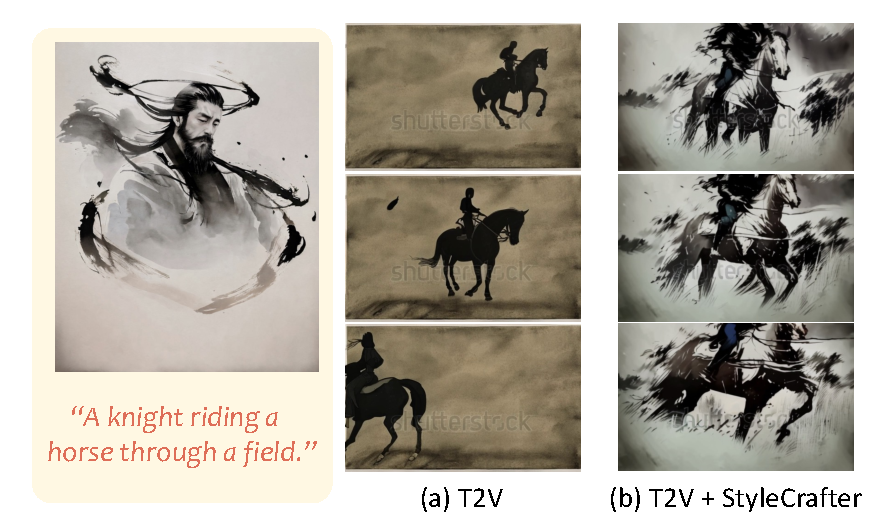
\includegraphics[width=\linewidth]{figures/motivation.pdf}\vspace{-0.5em}
%     \caption{Effect of adding style adapter to T2V models. (a) and (b) are results of Stable Diffusion~\cite{ldm} and VideoCrafter~\cite{chen2023videocrafter}. (c) is the result of VideoCrafter equipped with a style adapter. The content text prompt is "\textit{A knight riding a horse through the field}". For (a) and (b), the style prompt is generated from the style image using GPT4V~\cite{openai2023gpt4v}. \TODO{delete this figure}} 
%     \label{fig:motivation}\vspace{-0.5em}
% \end{figure}

In this paper, we propose StyleCrafter, a generic method that enhances pre-trained T2V models with a style control adapter, enabling text-to-video generation in any desired style by providing a reference image. 
% The advantages are twofold: (i) a style image offers stylistic feature guidance, complementing the stylization capabilities of T2V models in a zero-shot fashion; (ii) the reference image delivers a more accurate portrayal of the desired visual style compared to textual descriptions. 
Anyhow, it is non-trivial to achieve this goal. (i) as a classic problem of style transfer/preservation, the style control adapter requires to extract accurate style concepts from the reference image \textbf{in a content-style decoupled manner}. (ii) \textbf{the scarcity of open-source stylized videos} challenges the adaptation training of the T2V models.

Considering the scarcity of stylized videos, we propose to first train a style adapter to extract desired style concepts from images over image datasets, and then transfer the learned stylization ability to a T2V model with shared spatial weights through a tailor-made finetuning paradigm. The advantages are twofold: on the one hand, the adapter trained over stylized images can effectively extract the style concept from input images, eliminating the necessity for scarcely available stylized videos. On the other, a finetuning paradigm enables text-to-video models with better adaptation to the style concepts extracted from the previously trained style adapter, while avoiding degradation of temporal quality in video generation. 

To effectively capture the style features and promote content-style disentanglement, we adopt the widely used query transformer to extract style concepts from a single image. Particularly, we design a scale-adaptive fusion module to balance the influences of text-based content features and image-based style features, which helps generalization across various text and style combinations. During the training process, we employ carefully designed data augmentation strategies to enhance decoupled learning.

StyleCrafter efficiently generates high-quality stylized videos that align with the content of the texts and resemble the style of the reference images.
Comprehensive experiments are conducted to assess our proposed approach, demonstrating that it significantly outperforms existing competitors in both stylized image generation and stylized video generation. Furthermore, ablation studies offer a thorough analysis of the technical decisions made in developing the complete method, which provides valuable insights for the community.
Our contributions are summarized as follows:
\begin{itemize}
    \item We propose the concept of improving stylized generation for pre-trained T2V models by adding a style adapter.
    \item We explore an efficient network for stylized generation, which facilitates the content-style disentangled generation from text and image inputs. Our method attains notable advantages over existing baselines.
    \item We propose a training paradigm for generic T2V style adapter without requiring any stylized videos for supervision.
\end{itemize}
\section{Alternative Explanation for Emergent Abilities}
\label{sec:alt_explanation}

\begin{figure}
    \centering
    % 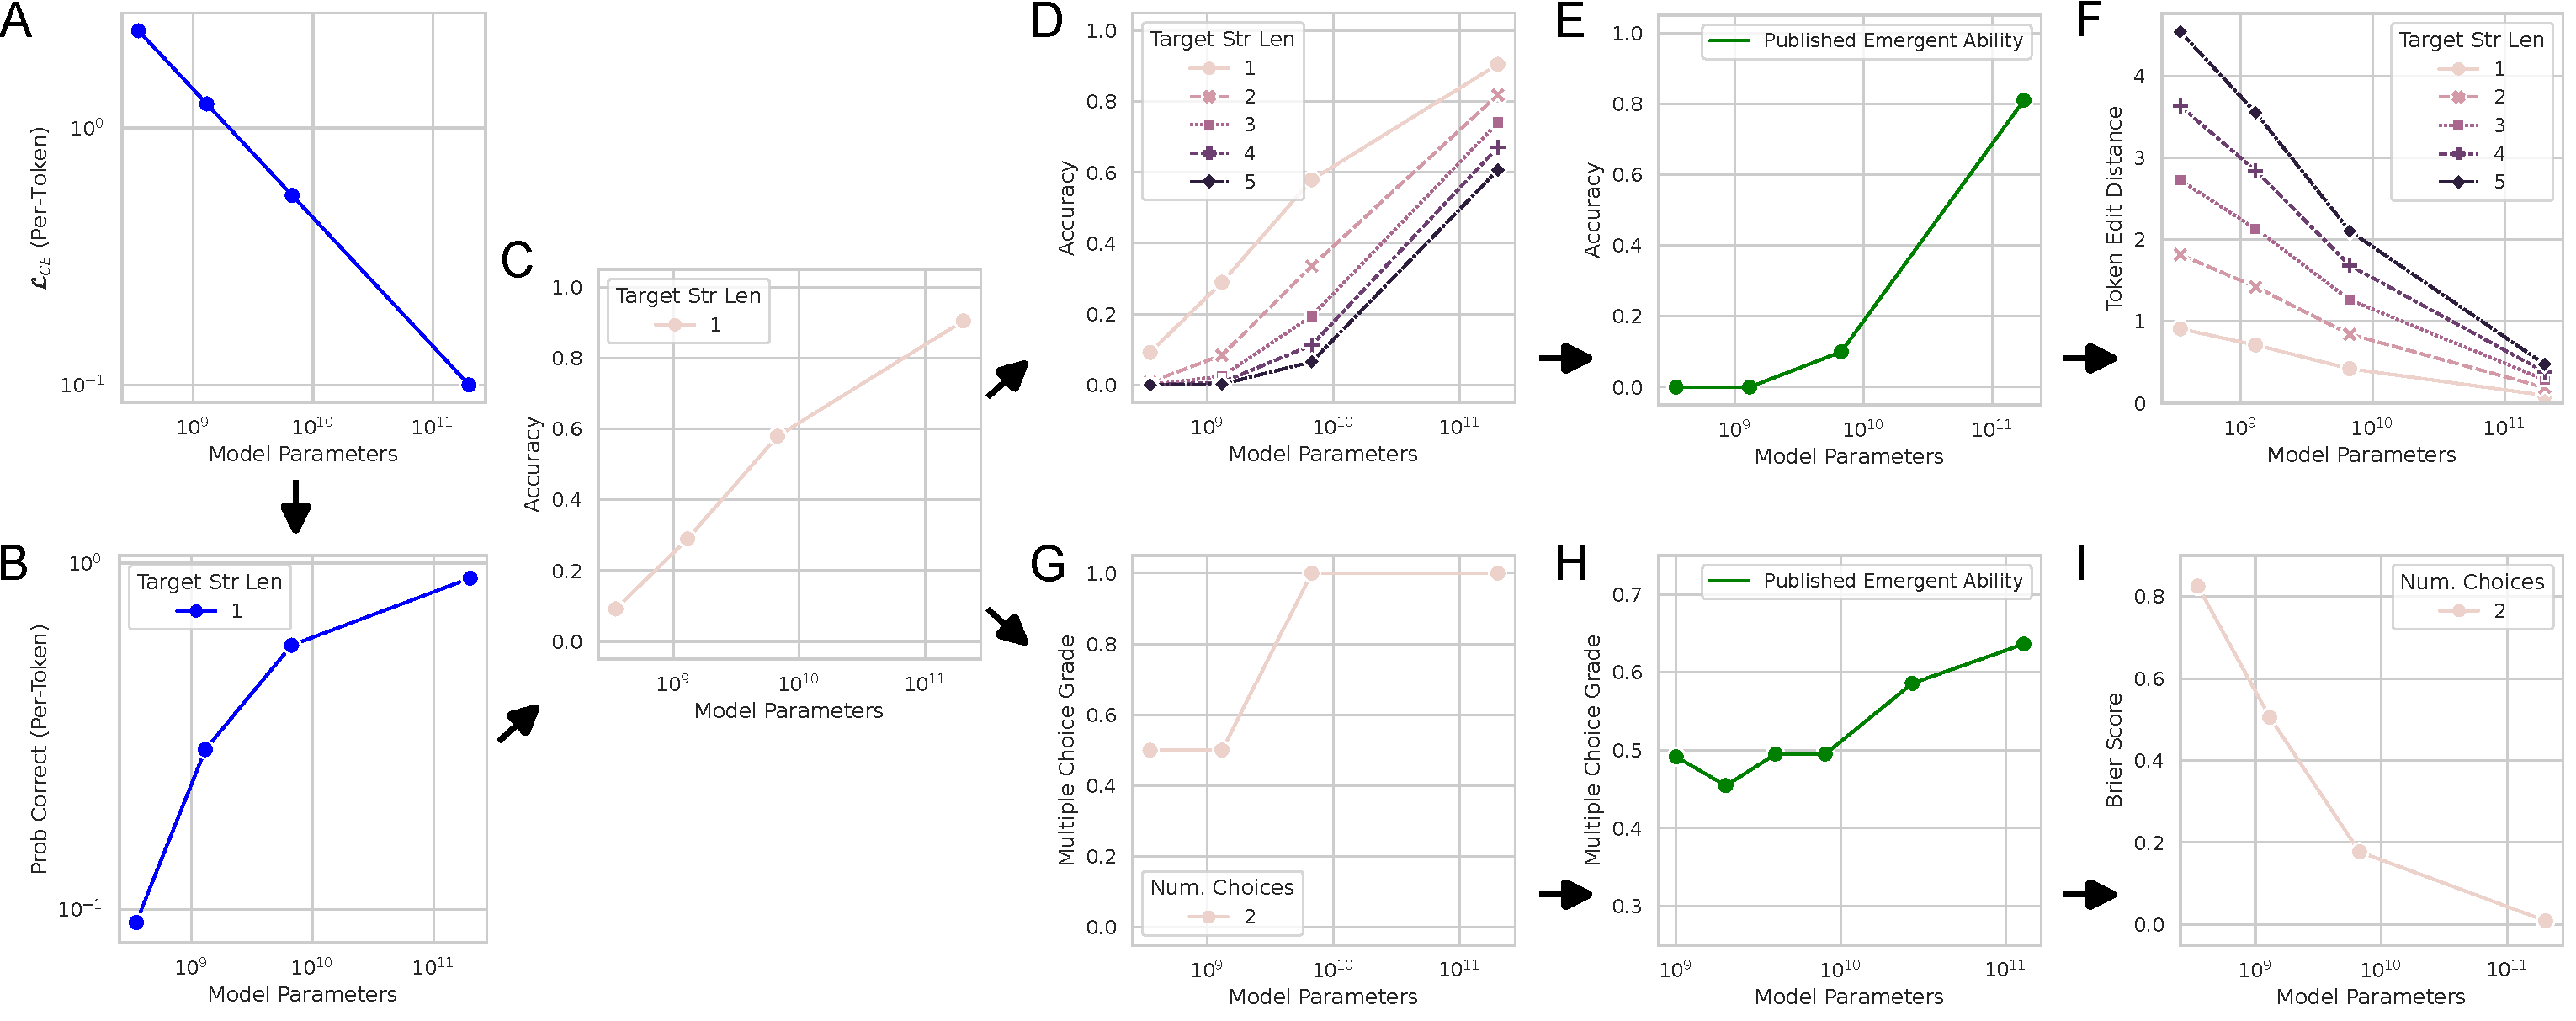
\includegraphics[width=\textwidth]{figures/toy_emergence/toy_analytical_model.pdf}
    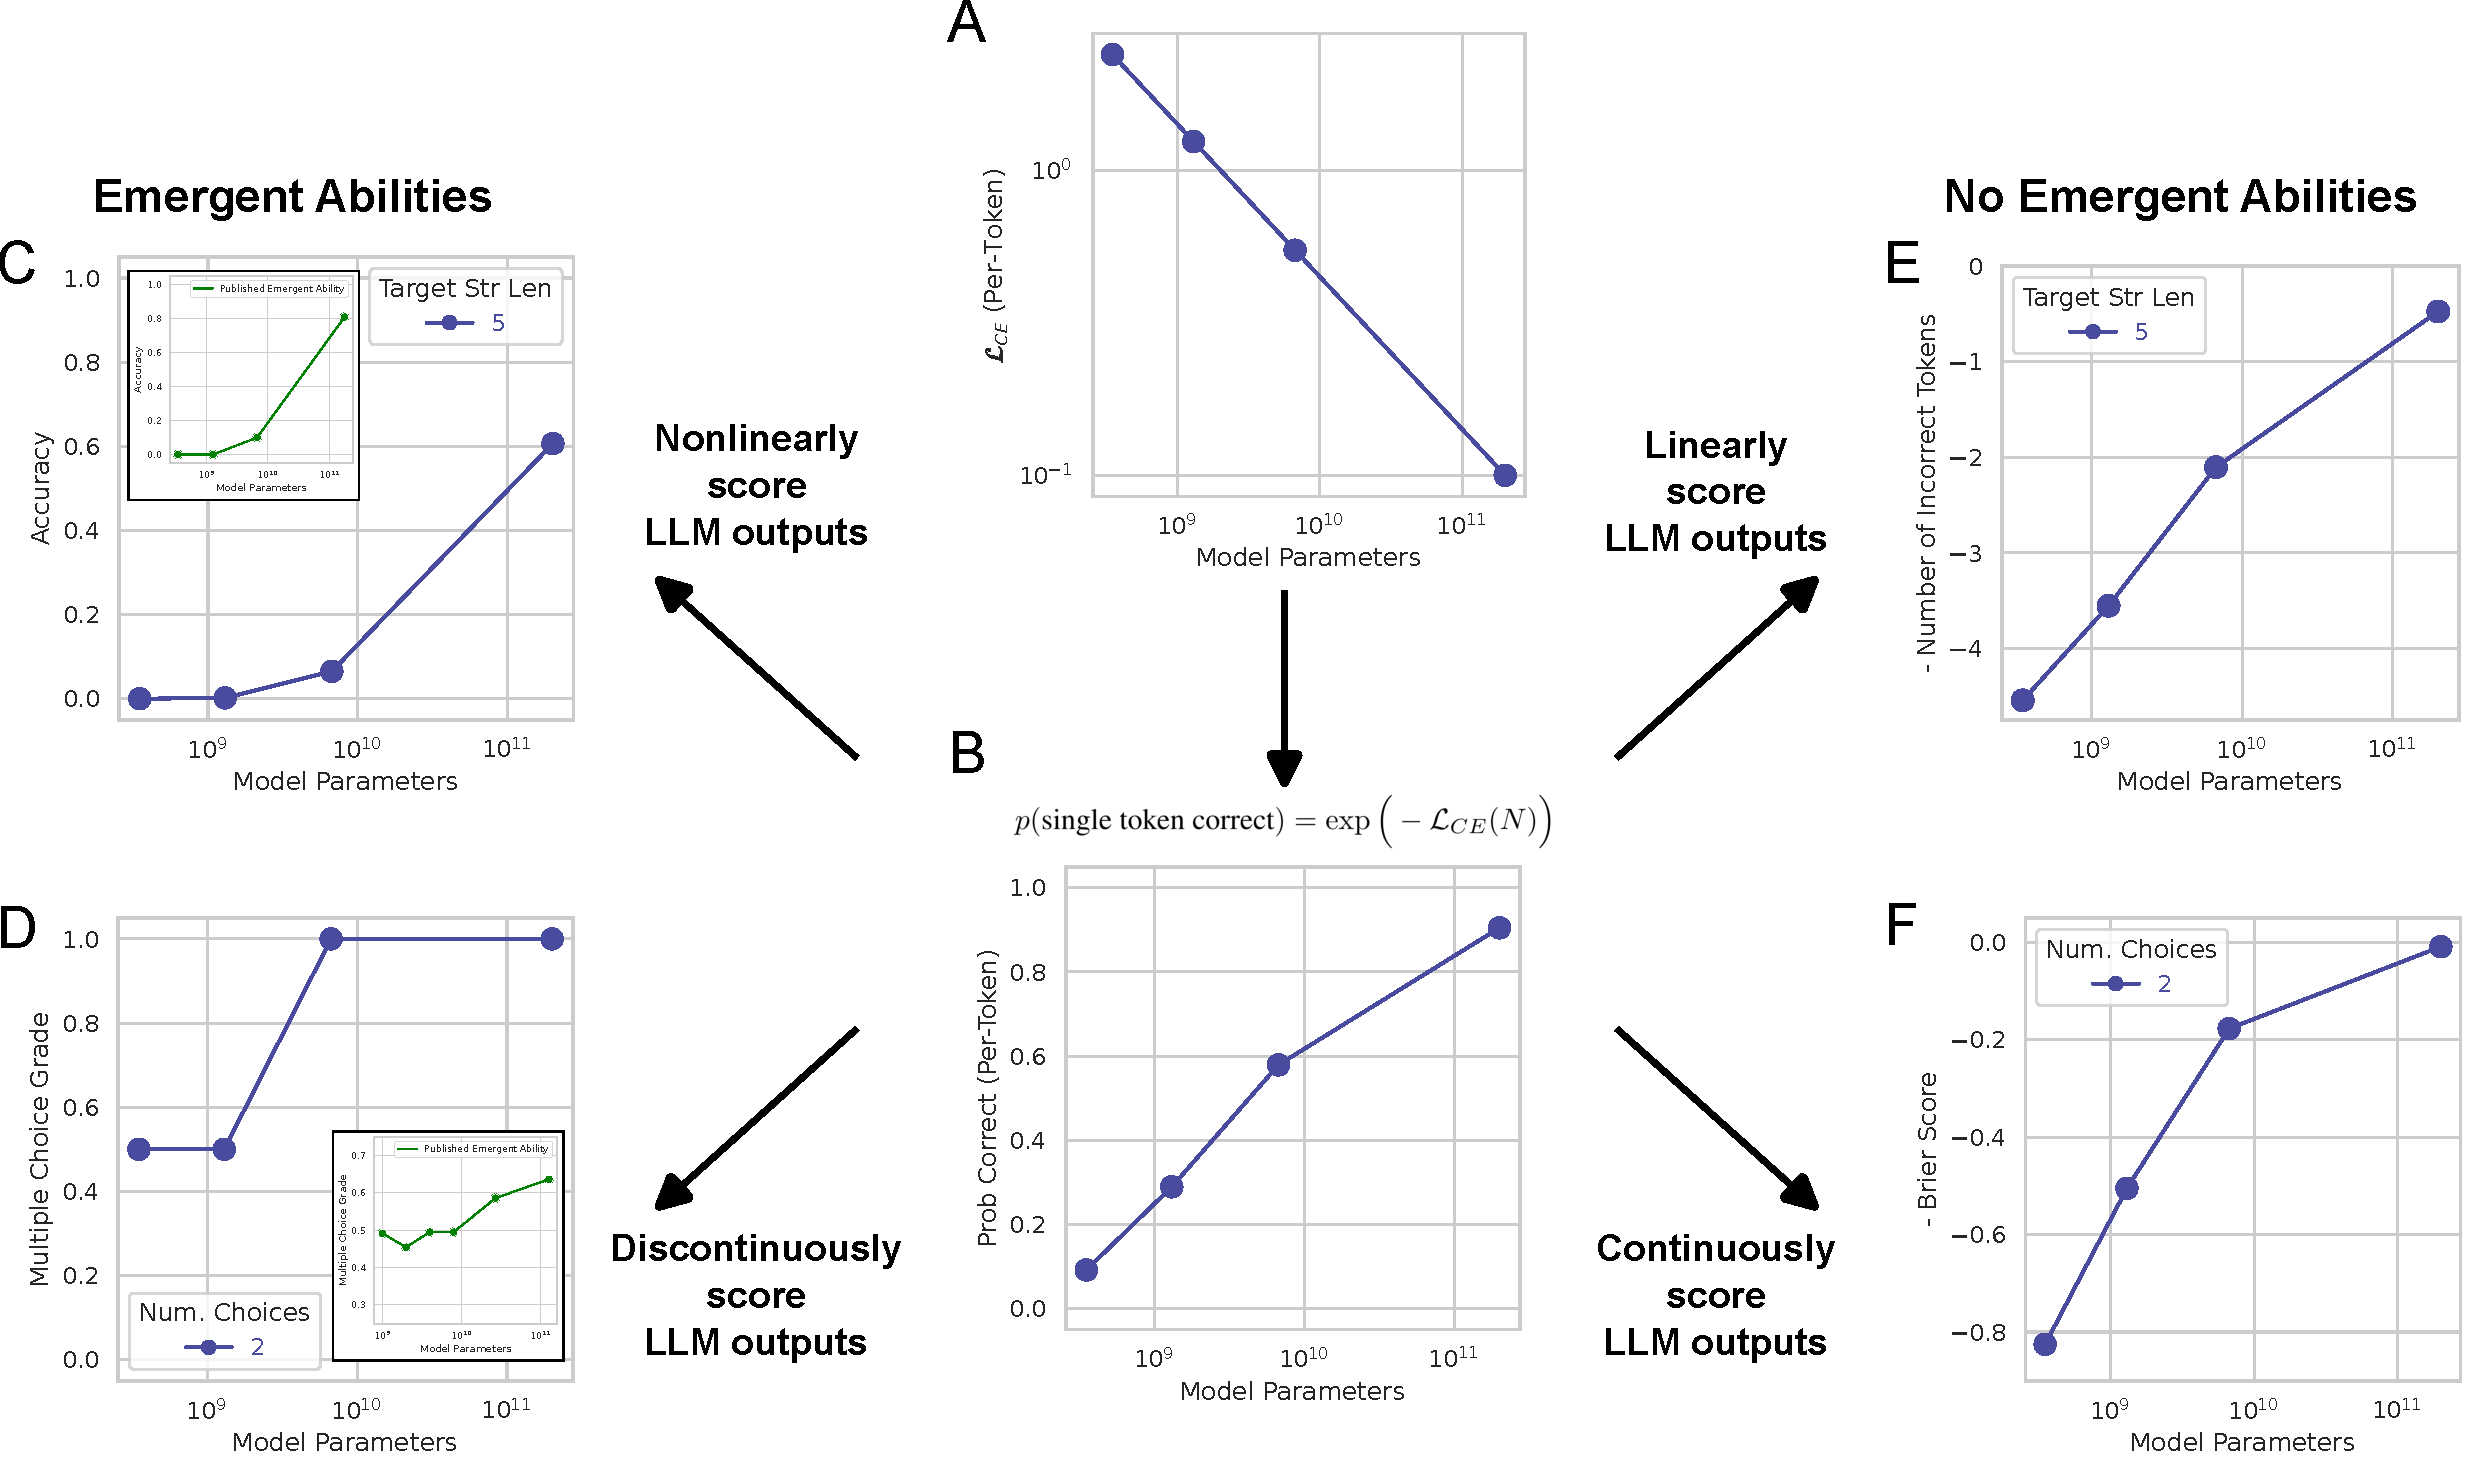
\includegraphics[width=0.9\textwidth]{figures/toy_emergence/toy_analytical_model_try2.pdf}
    \caption{\textbf{Emergent abilities of large language models are created by the researcher's chosen metrics, not unpredictable changes in model behavior with scale.} (A) Suppose the per-token cross-entropy loss decreases monotonically with model scale, e.g., $\mathcal{L}_{CE}$ scales as a power law. (B) The per-token probability of selecting the correct token asymptotes towards 1. (C) If the researcher scores models' outputs using a nonlinear metric such as Accuracy (which requires a sequence of tokens to \textit{all} be correct), the metric choice nonlinearly scales performance, causing performance to change sharply and unpredictably in a manner that qualitatively matches published emergent abilities (inset). (D) If the researcher instead scores models' outputs using a discontinuous metric such as Multiple Choice Grade (akin to a step function), the metric choice discontinuously scales performance, again causing performance to change sharply and unpredictably. (E) Changing from a nonlinear metric to a linear metric such as Token Edit Distance, scaling shows smooth, continuous and predictable improvements, ablating the emergent ability. (F) Changing from a discontinuous metric to a continuous metric such as Brier Score again reveals smooth, continuous and predictable improvements in task performance. Consequently, emergent abilities are created by the researcher's choice of metrics, not fundamental changes in model family behavior on specific tasks with scale.}
    \label{fig:toy_model}
\end{figure}

How might smooth, continuous, predictable changes in model family performance appear sharp and unpredictable?
% The answer is that even if the per-token error rate changes smoothly with scale, the researcher's choice of a nonlinear or discontinuous metric can distort the model family's performance to appear sharp and unpredictable.
The answer is that the researcher's choice of a nonlinear or discontinuous metric can distort the model family's performance to appear sharp and unpredictable.

To expound, suppose that within a model family, the test loss falls smoothly, continuously and predictably with the number of model parameters.
One reason to believe this is the phenomenon known as neural scaling laws: empirical observations that deep networks exhibit power law scaling in the test loss as a function of training dataset size, number of parameters or compute \citep{hestness2017deep,rosenfeld2019constructive,henighan2020scaling,kaplan2020scaling,gordon2021data,hernandez2021scaling,jones2021scaling,zhai2022scaling,hoffmann2022training, clark2022unified, neumann2022scaling}.
%this finding has been observed spanning 7 orders of magnitude across diverse domains including vision and language modeling.
%Motivated by neural scaling laws, 
For concreteness, suppose we have a model family of different numbers of parameters $N > 0$ and assume that each model's per-token cross entropy falls as a power law with the number of parameters $N$ for constants $c > 0, \alpha < 0$ (Fig. \ref{fig:toy_model}A):

\begin{equation*}
    \mathcal{L}_{CE}(N) = \Big(\frac{N}{c}\Big)^{\alpha}
\end{equation*}

To be clear, we do not require this particular functional form to hold; rather, we use it for illustrative purposes.
Let $V$ denote the set of possible tokens, $p \in \Delta^{|V|-1}$ denote the true but unknown probability distribution, and $\hat{p}_N \in \Delta^{|V|-1}$ denote the $N$-parameter model's predicted probability distribution.
The per-token cross entropy as a function of number of parameters $N$ is:

\begin{equation*}
    \mathcal{L}_{CE}(N) \; \defeq \; - \sum_{v \in V} p(v) \log \hat{p}_N(v)
\end{equation*}

In practice, $p$ is unknown, so we substitute a one-hot distribution of the observed token $v^*$:

\begin{equation*}
    \mathcal{L}_{CE}(N) = - \log \hat{p}_N(v^*)
\end{equation*}

A model with $N$ parameters then has a per-token probability of selecting the correct token (Fig. \ref{fig:toy_model}B):

\begin{equation*}
    p(\text{single token correct}) = \exp \Big(- \mathcal{L}_{CE}(N) \Big) =\exp \Big(- (N/c)^{\alpha} \Big)
\end{equation*}

%As a  sanity check, note that as the number of parameters increases (decreases), the per-token accuracy asymptotes towards 1 (towards 0).
Suppose the researcher then chooses a metric that requires selecting $L$ tokens correctly.
For example, our task might be $L$-digit integer addition, and a model's output is scored $1$ if all $L$ output digits exactly match all target digits with no additions, deletions or substitutions, $0$ otherwise.
If the probability each token is correct is independent\footnote{While the independence assumption is not true, the approximation yields results qualitatively matching the observed emergence claims.}, the probability of scoring $1$ is:

\begin{equation*}
    \text{Accuracy}(N) \approx p_N(\text{single token correct})^{\text{num. of tokens}} = \exp \Big(- (N/c)^{\alpha} \Big)^L
\end{equation*}

This choice of metric nonlinearly scales performance with increasing token sequence length. When plotting performance on a linear-log plot, one sees a sharp, unpredictable emergent ability on longer sequences  (Fig. \ref{fig:toy_model}C) that closely matches claimed emergent abilities (inset).
What happens if the researcher switches from a nonlinear metric like Accuracy, under which the per-token error rate scales geometrically in target length (App. \ref{app:metric_scaling:accuracy}), to an approximately linear metric like Token Edit Distance, under which the per-token error rate scales quasi-linearly in target length (App. \ref{app:metric_scaling:token_edit_distance})?

\begin{equation*}
    \text{Token Edit Distance}(N) \approx L \, \Big(1 - p_N(\text{single token correct}) \Big) = L \, \Big( 1 - \exp \big(- (N/c)^{\alpha} \big) \Big)
\end{equation*}

The linear metric reveals smooth, continuous, predictable changes in model performance (Fig. \ref{fig:toy_model}E).
Similarly, if the researcher uses a discontinuous metric like Multiple Choice Grade, the researcher can find emergent abilities (Fig. \ref{fig:toy_model}D), but switching to a continuous metric like Brier Score removes the emergent ability (Fig. \ref{fig:toy_model}F).
In summary, sharp and unpredictable changes with increasing scale can be fully explained by three interpretable factors: (1) the researcher choosing a metric that nonlinearly or discontinuously scales the per-token error rate, (2) having insufficient resolution to estimate model performance in the smaller parameter regime, with resolution\footnote{Resolution is defined as ``The smallest interval measurable by a scientific instrument; the resolving power."} set by $1/\text{test dataset size}$, and (3) insufficiently sampling the larger parameter regime. 
\section{Analyzing InstructGPT/GPT-3's Emergent Arithmetic Abilities}

\begin{figure}
    \centering
    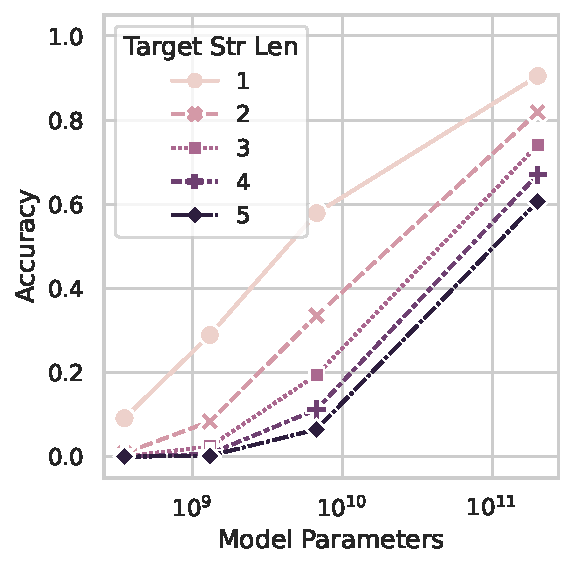
\includegraphics[width=0.26\textwidth]{figures/toy_emergence/acc_many_vs_model_size_by_target_str_len.pdf}%
    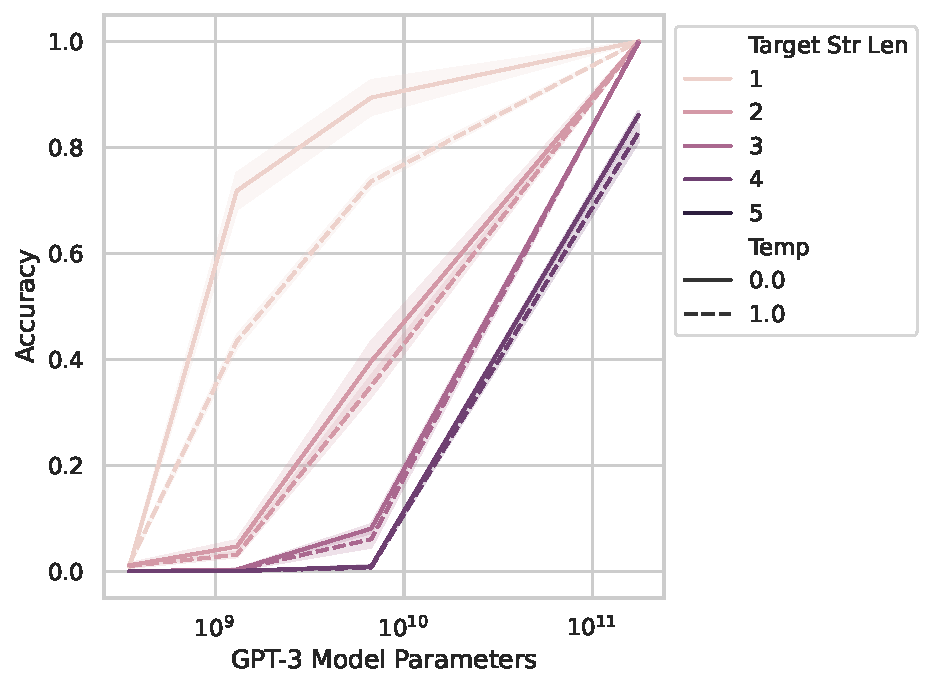
\includegraphics[width=0.35\textwidth]{figures/gpt3_integer_multiplication/multiplication_acc_vs_model_size_by_temp_by_target_str_len.pdf}%
    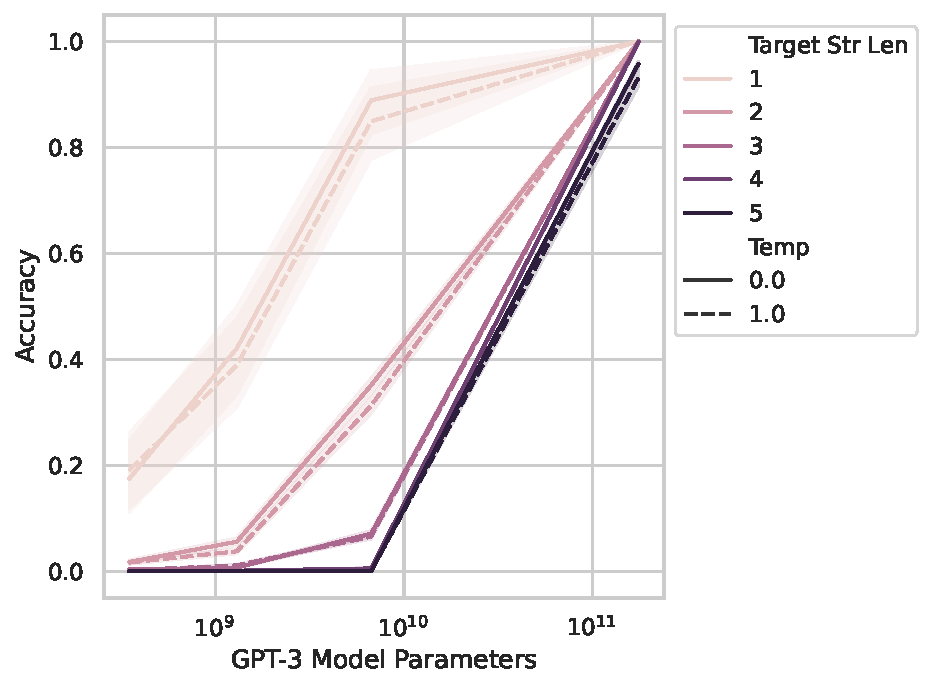
\includegraphics[width=0.35\textwidth]{figures/gpt3_integer_addition/addition_acc_vs_model_size_by_temp_by_target_str_len.pdf}
    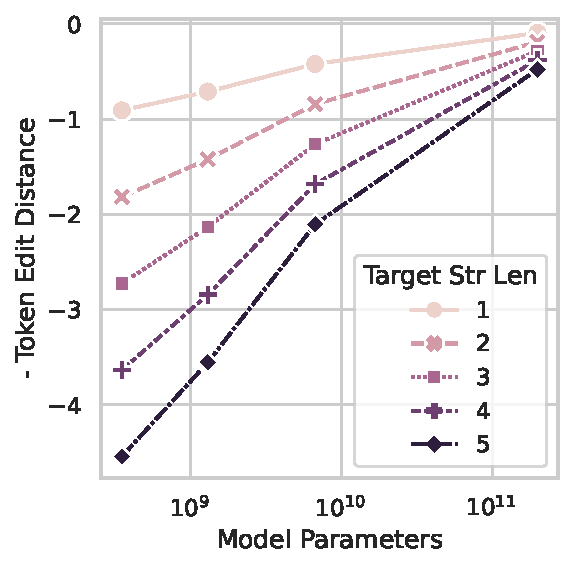
\includegraphics[width=0.26\textwidth]{figures/toy_emergence/neg_token_edit_dist_many_vs_model_size_by_target_str_len.pdf}%
    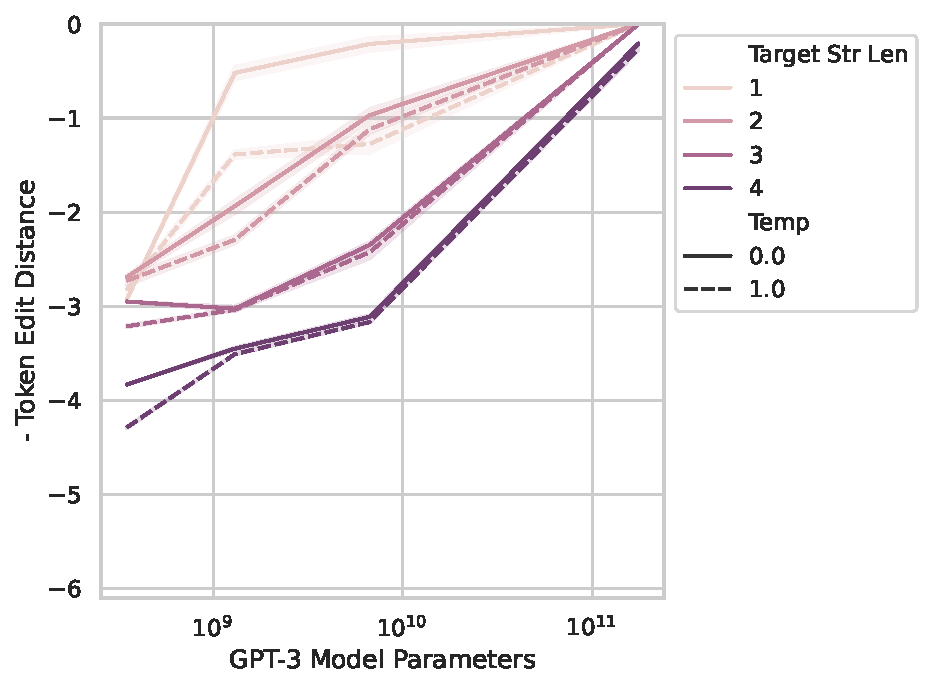
\includegraphics[width=0.35\textwidth]{figures/gpt3_integer_multiplication/multiplication_neg_token_edit_dist_vs_model_size_by_temp_by_target_str_len.pdf}%
    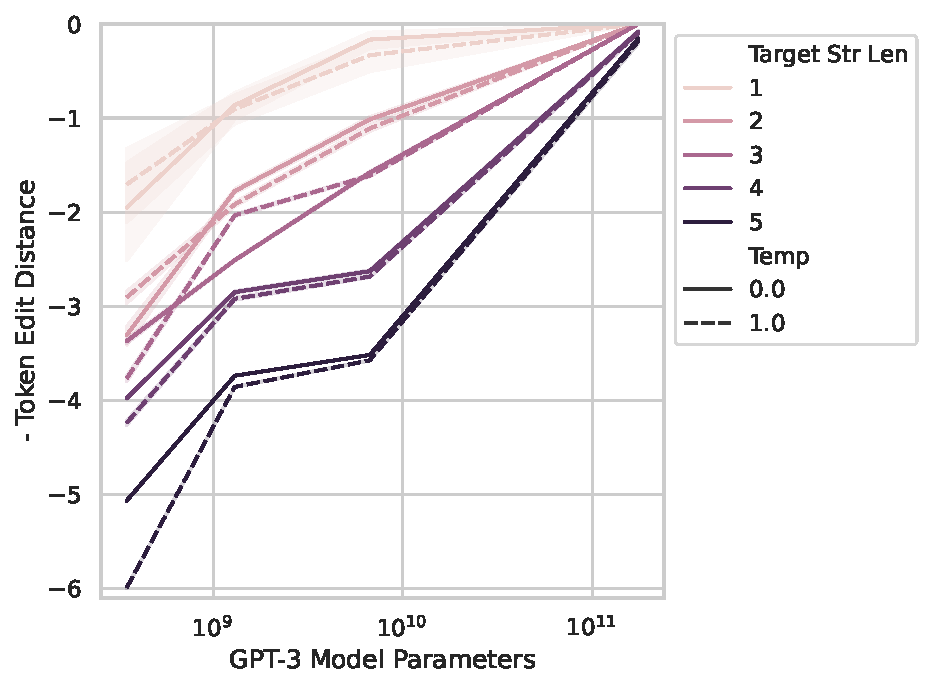
\includegraphics[width=0.35\textwidth]{figures/gpt3_integer_addition/addition_neg_token_edit_dist_vs_model_size_by_temp_by_target_str_len.pdf}
    \caption{\textbf{Claimed emergent abilities evaporate upon changing the metric.} Left to Right: Mathematical Model, 2-Integer 2-Digit Multiplication Task, 2-Integer 4-Digit Addition Task. Top: When performance is measured by a nonlinear metric (e.g., Accuracy), the InstructGPT/GPT-3 \cite{brown2020language, lowe2022instruct} family's performance appears sharp and unpredictable on longer target lengths. Bottom: When performance is instead measured by a linear metric (e.g., Token Edit Distance), the family exhibits smooth, predictable performance improvements.
    %for two claimed emergent abilities.
    }
    \label{fig:gpt_metric_change}
\end{figure}

Previous papers prominently claimed the GPT \cite{brown2020language,lowe2022instruct} family\footnote{As of 2023-03-15, 4 models with 350M, 1.3B,  6.7B, 175B parameters are available via the OpenAI API.} displays emergent abilities at integer arithmetic tasks \cite{ganguli2022predictability, srivastava2022beyond,wei2022emergent} (Fig. \ref{fig:toy_model}E).
We chose these tasks as they were prominently presented \cite{brown2020language,ganguli2022predictability,srivastava2022beyond,wei2022emergent}, and we focused on the GPT family due to it being publicly queryable.
As explained mathematically and visually in Sec. \ref{sec:alt_explanation}, our alternative explanation makes three predictions:
%
\begin{enumerate}
    \item Changing the metric from a nonlinear or discontinuous metric (Fig. \ref{fig:toy_model}CD) to a linear or continuous metric (Fig. \ref{fig:toy_model} EF) should reveal smooth, continuous, predictable performance improvement with model scale.
    \item For nonlinear metrics, increasing the resolution of measured model performance by increasing the test dataset size should reveal smooth, continuous, predictable model improvements \textit{commensurate with the predictable nonlinear effect of the chosen metric}.
    \item Regardless of metric, increasing the target string length should predictably affect the model's performance as a function of the length-1 target performance: approximately geometrically for accuracy and approximately quasilinearly for token edit distance.
\end{enumerate}

To test these predictions, we collected outputs from the InstructGPT/GPT-3 family on two tasks: 2-shot multiplication between two 2-digit integers and 2-shot addition between two 4-digit integers.
% We chose 2-shot prompting arbitrarily and were unable to experiment more broadly due to financial constraints.

\begin{figure}
    \centering
    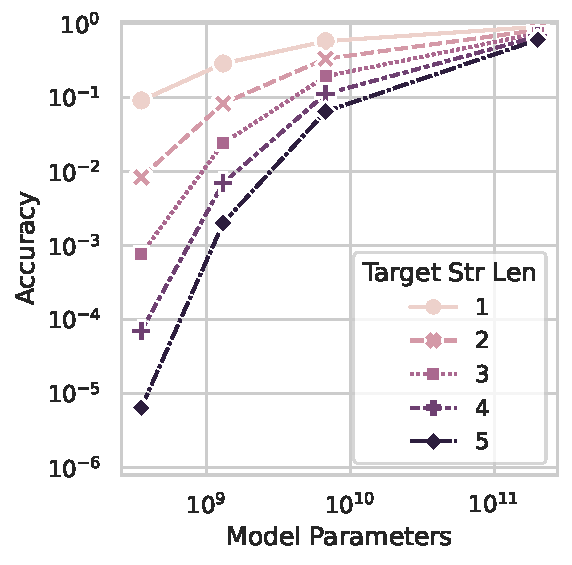
\includegraphics[width=0.26\textwidth]{figures/toy_emergence/acc_log_many_vs_model_size_by_target_str_len.pdf}%
    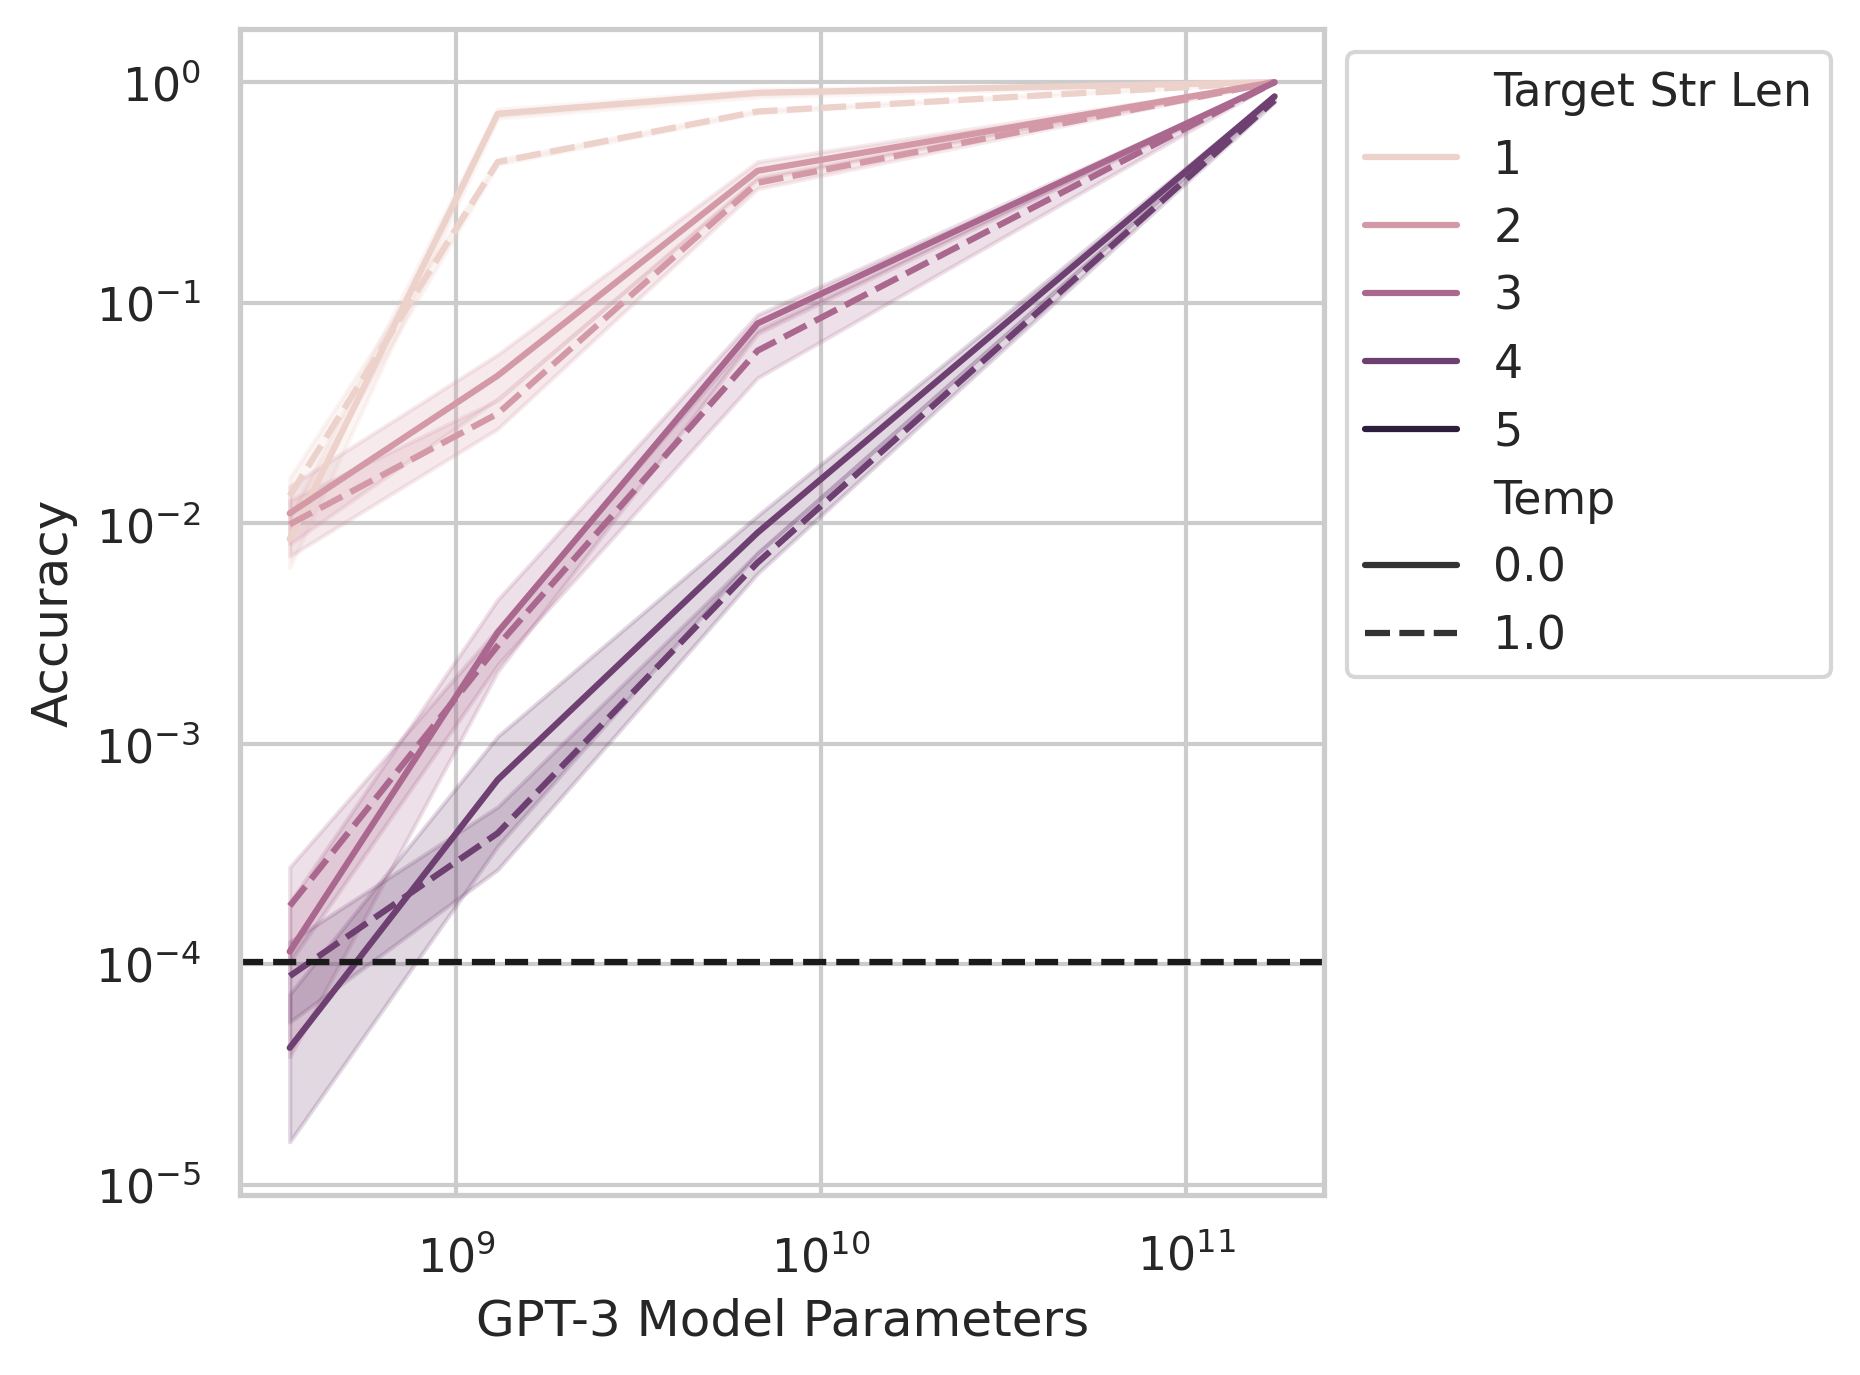
\includegraphics[width=0.35\textwidth]{figures/gpt3_integer_multiplication/multiplication_acc_log_vs_model_size_by_temp_by_target_str_len.png}%
    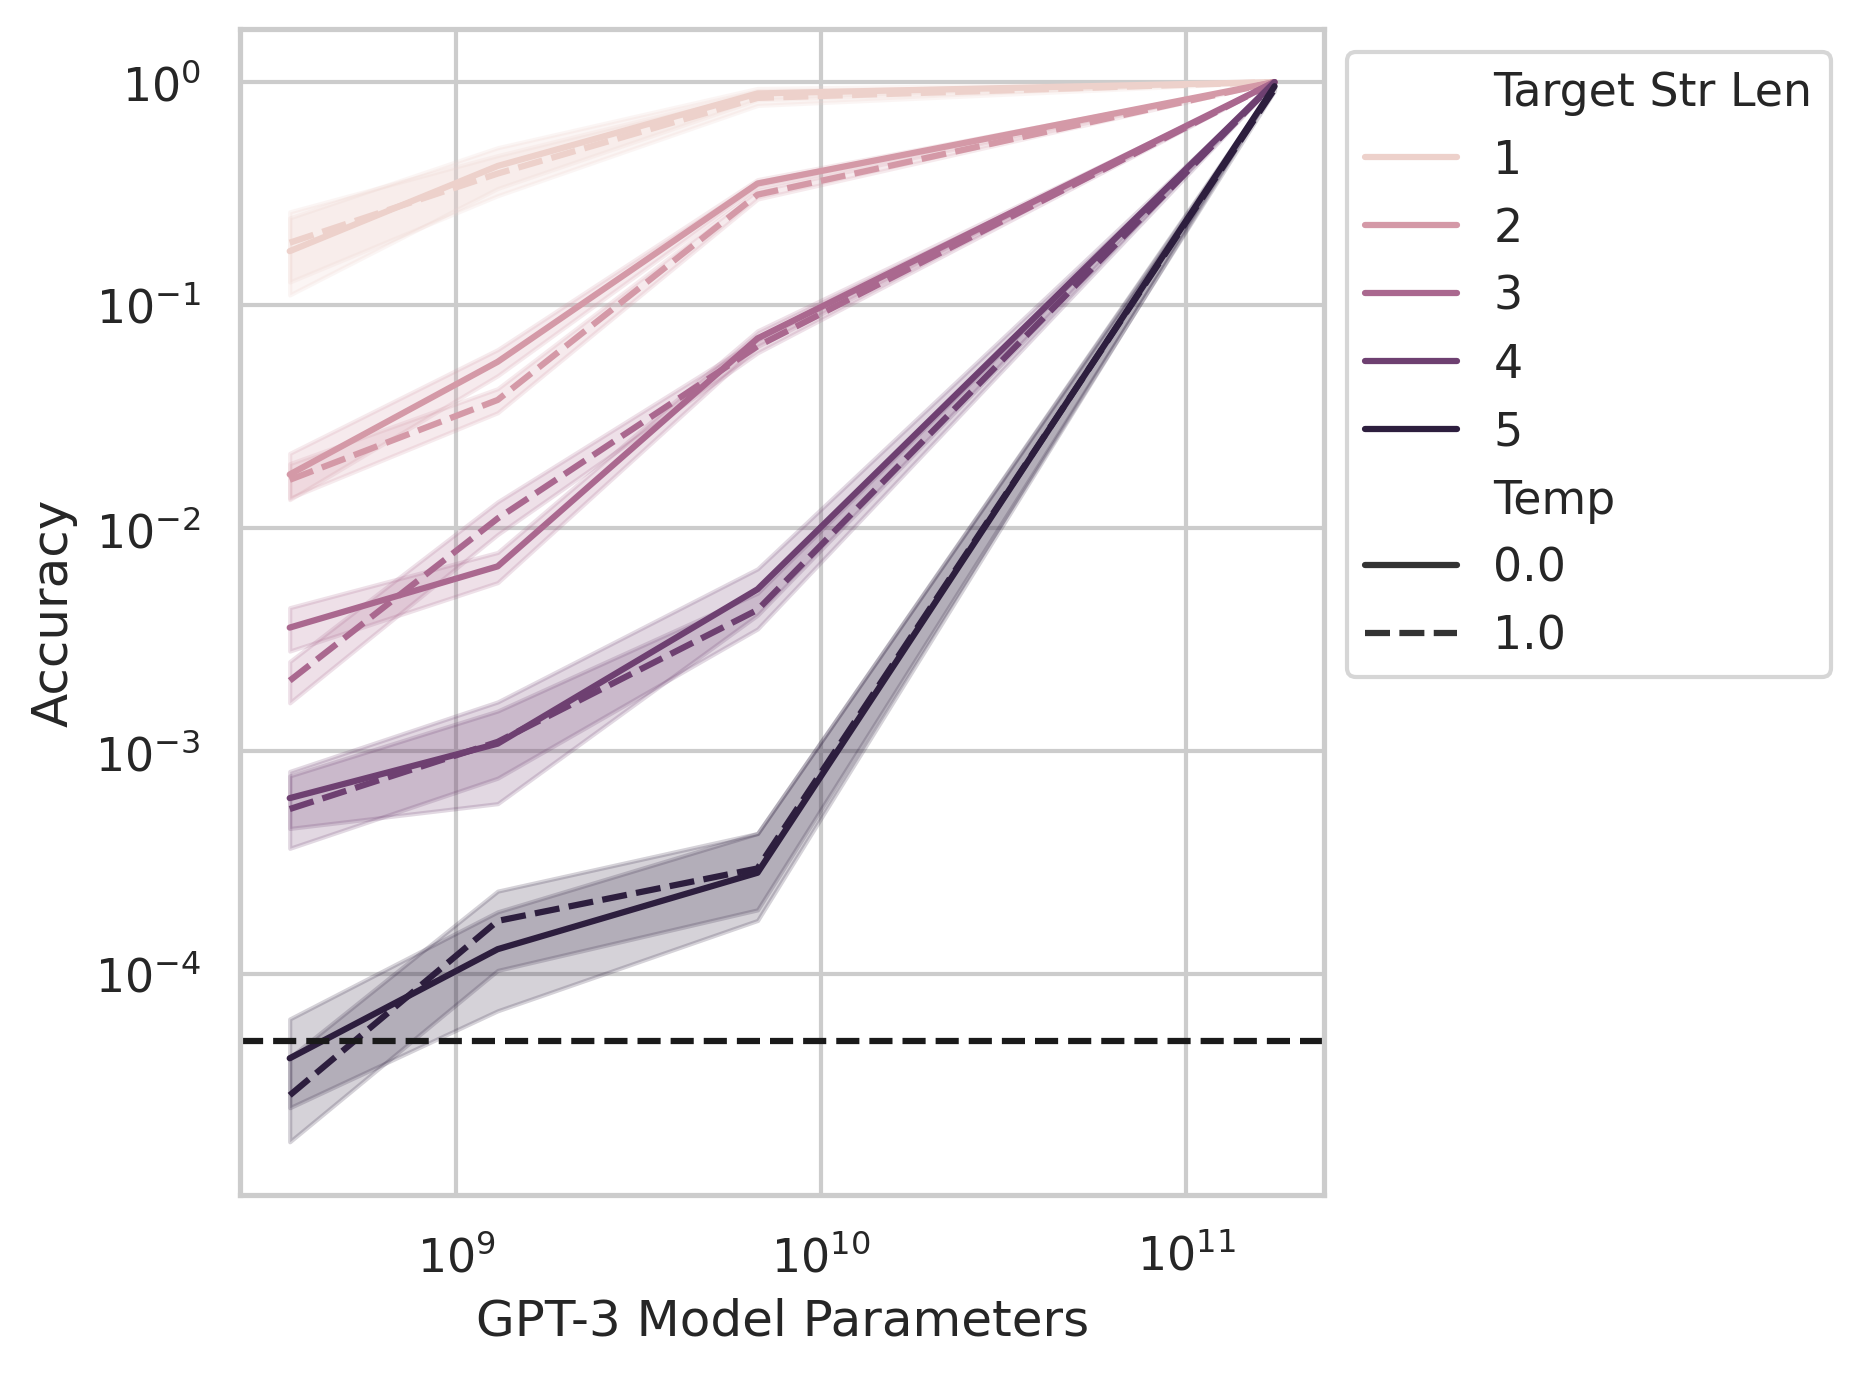
\includegraphics[width=0.35\textwidth]{figures/gpt3_integer_addition/addition_acc_log_vs_model_size_by_temp_by_target_str_len.png}
    \caption{\textbf{Claimed emergent abilities evaporate upon using better statistics.} Left to Right: Mathematical Model, 2-Integer 2-Digit Multiplication Task, 2-Integer 4-Digit Addition Task. Based on the predictable effect Accuracy has on performance, measuring performance requires high resolution. Generating additional test data increases the resolution and reveals that even on Accuracy, the InstructGPT/GPT-3 family's \cite{brown2020language, lowe2022instruct} performance is above chance and improves in a smooth, continuous, predictable manner that qualitatively matches the mathematical model.}
    \label{fig:gpt_improve_resolution}
\end{figure}

% \begin{figure}
%     \centering
%     \begin{center}
%         4-Digit Integer Addition \quad \quad \quad \quad \quad \quad 2-Digit Integer Multiplication
%     \end{center}
%     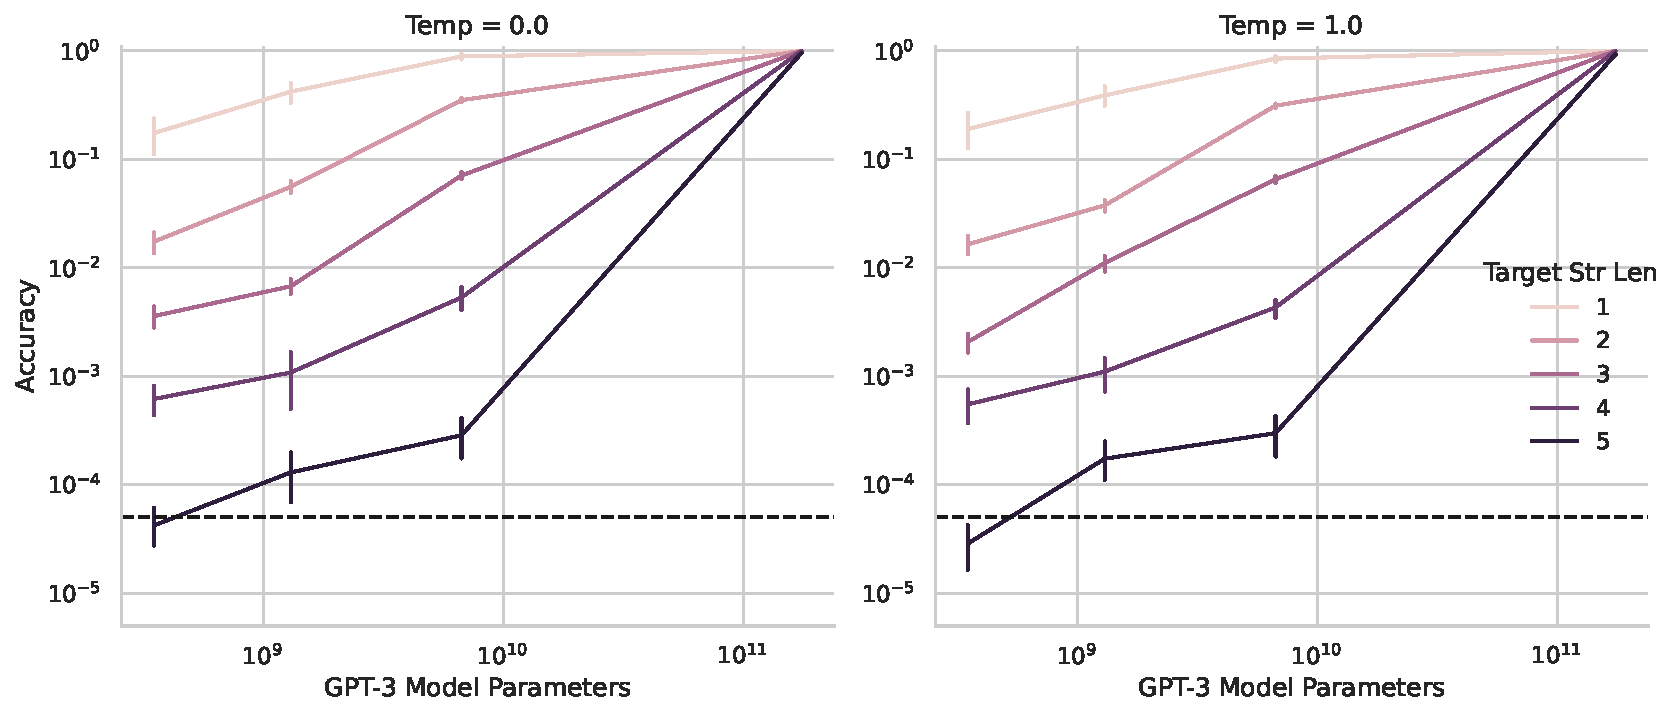
\includegraphics[width=0.49\textwidth]{figures/gpt3_integer_addition/addition_acc_vs_model_size_by_target_str_len.pdf}
%     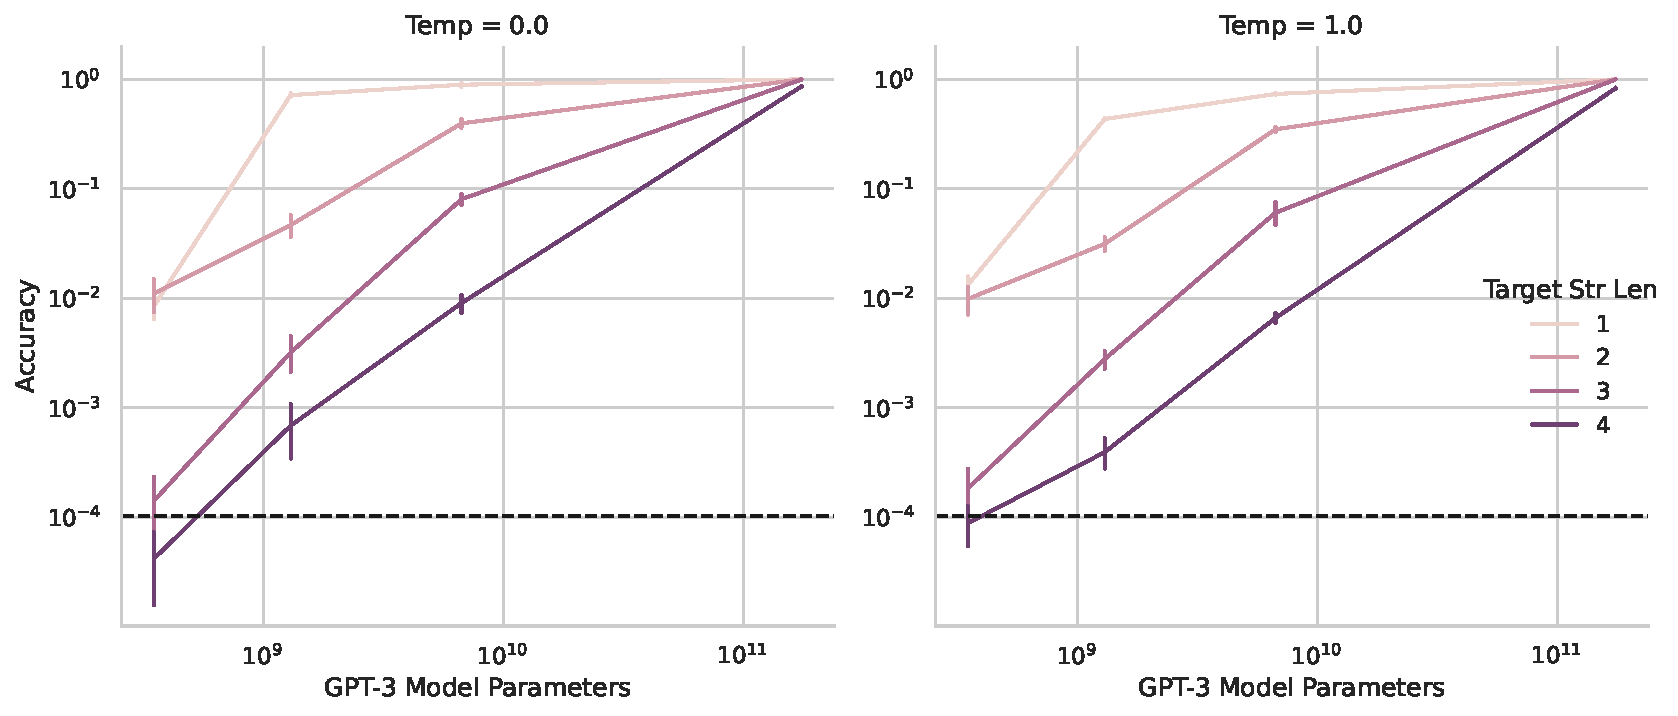
\includegraphics[width=0.49\textwidth]{figures/gpt3_integer_multiplication/multiplication_acc_vs_model_size_by_target_str_len.pdf}
%     \caption{\textbf{Better estimating accuracy with more test data reveals that performance changes are smooth, continuous and predictable}.}
%     \label{fig:gpt_improve_resolution}
% \end{figure}


\paragraph{Prediction: Emergent Abilities Disappear With Different Metrics}
On both arithmetic tasks, the GPT family displays emergent abilities if the target has 4 or 5 digits and if the metric is Accuracy (Fig. \ref{fig:gpt_metric_change}, top) \cite{brown2020language, ganguli2022predictability,wei2022emergent}. However, if one changes from nonlinear Accuracy to linear Token Edit Distance \textit{while keeping the models' outputs fixed}, the family's performance smoothly, continuously and predictably improves with increasing scale (Fig. \ref{fig:gpt_metric_change}, bottom). This confirms our first prediction and supports our alternative explanation that the source of emergent abilities is the researcher's choice of metric, \textit{not changes in the model family's outputs}. We also observe that under Token Edit Distance, increasing the length of the target string from 1 to 5 predictably decreases the family's performance in an approximately quasilinear manner, confirming the first half of our third prediction.

% \begin{figure}
%     \centering
%     \begin{minipage}{.25\textwidth}
%         \centering
%         Mathematical Model
%         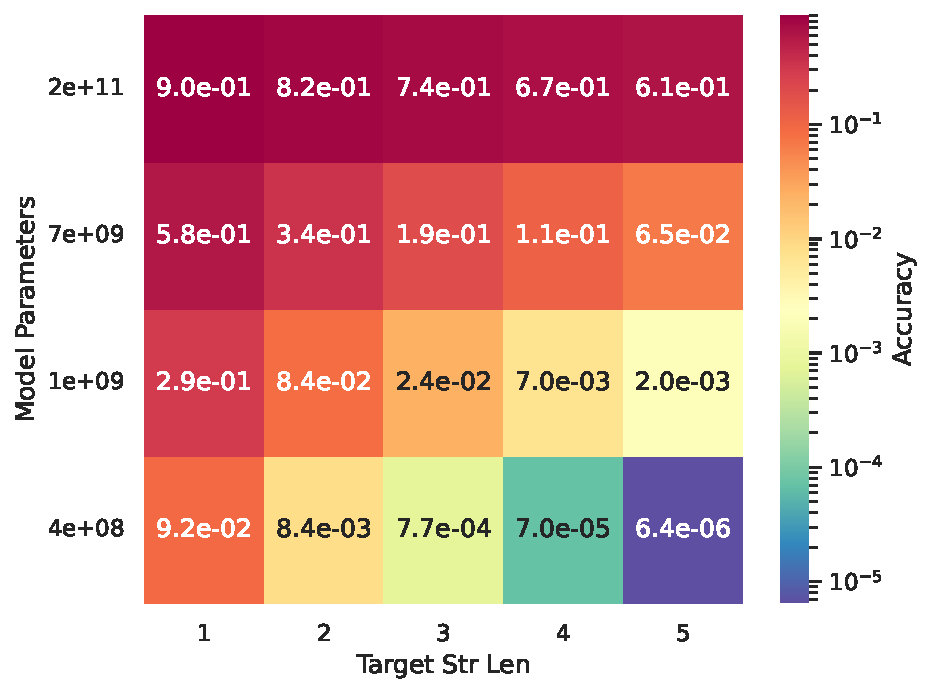
\includegraphics[width=0.95\textwidth]{figures/toy_emergence/heatmap_acc_by_model_size_by_target_str_len.pdf}
%     \end{minipage}\hfill
%     \begin{minipage}{0.36\textwidth}
%         \centering
%         4-Digit Integer Addition
%         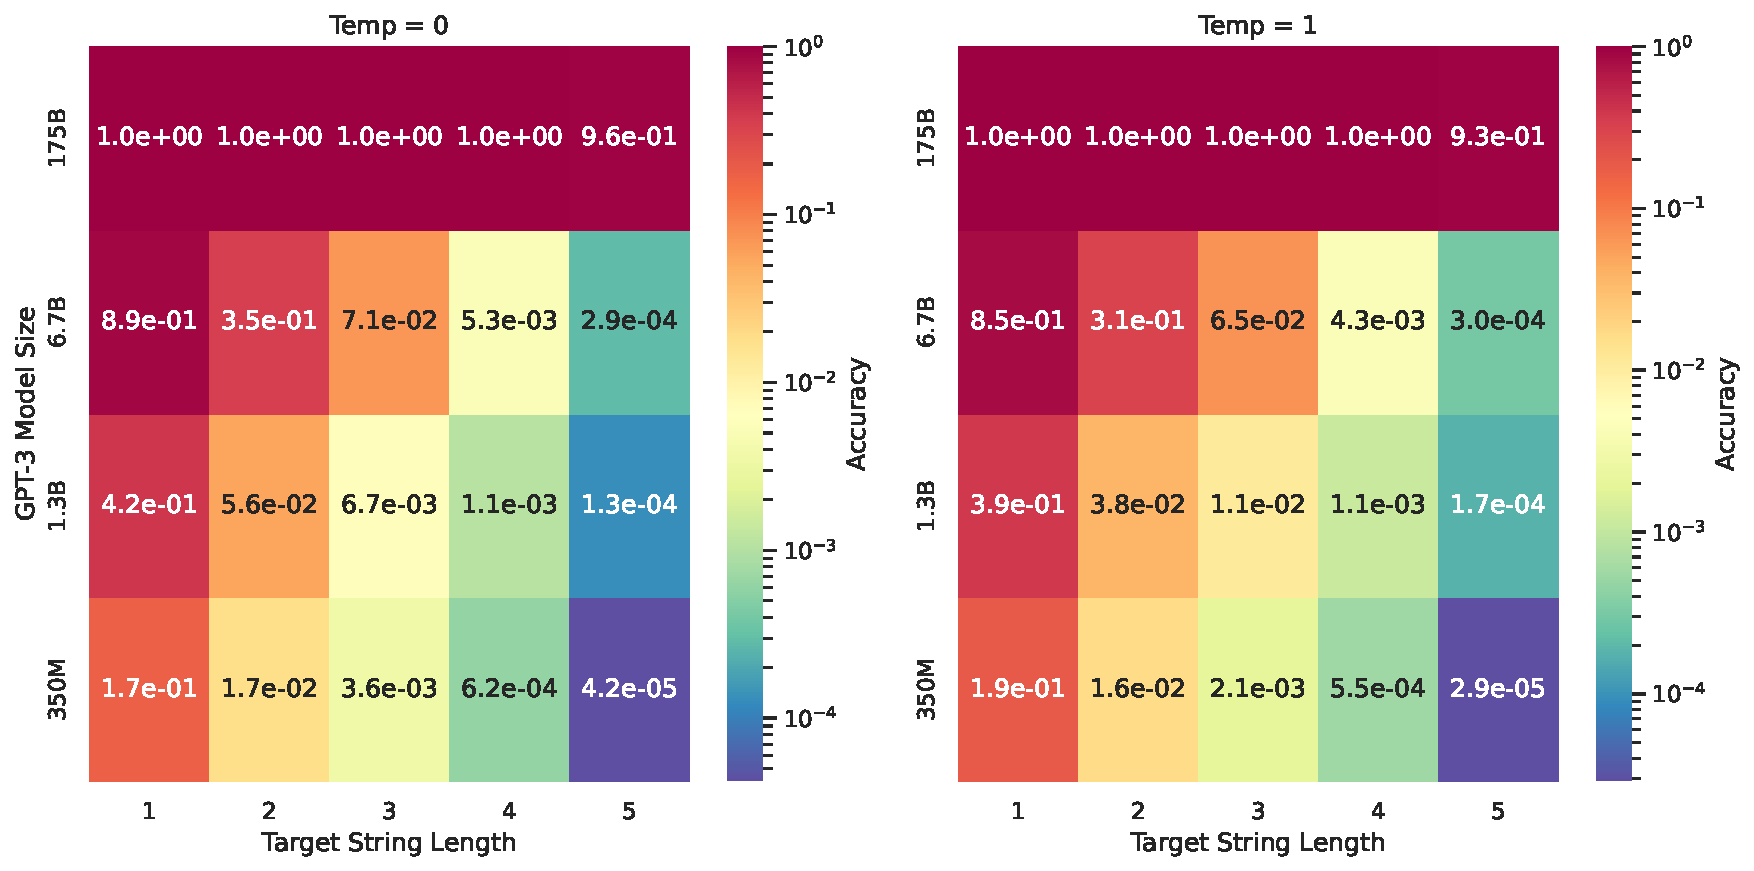
\includegraphics[width=0.95\textwidth]{figures/gpt3_integer_addition/heatmap_acc_by_model_size_by_target_str_len.pdf}
%     \end{minipage}\hfill
%     \begin{minipage}{0.36\textwidth}
%         \centering
%         2-Digit Integer Multiplication
%         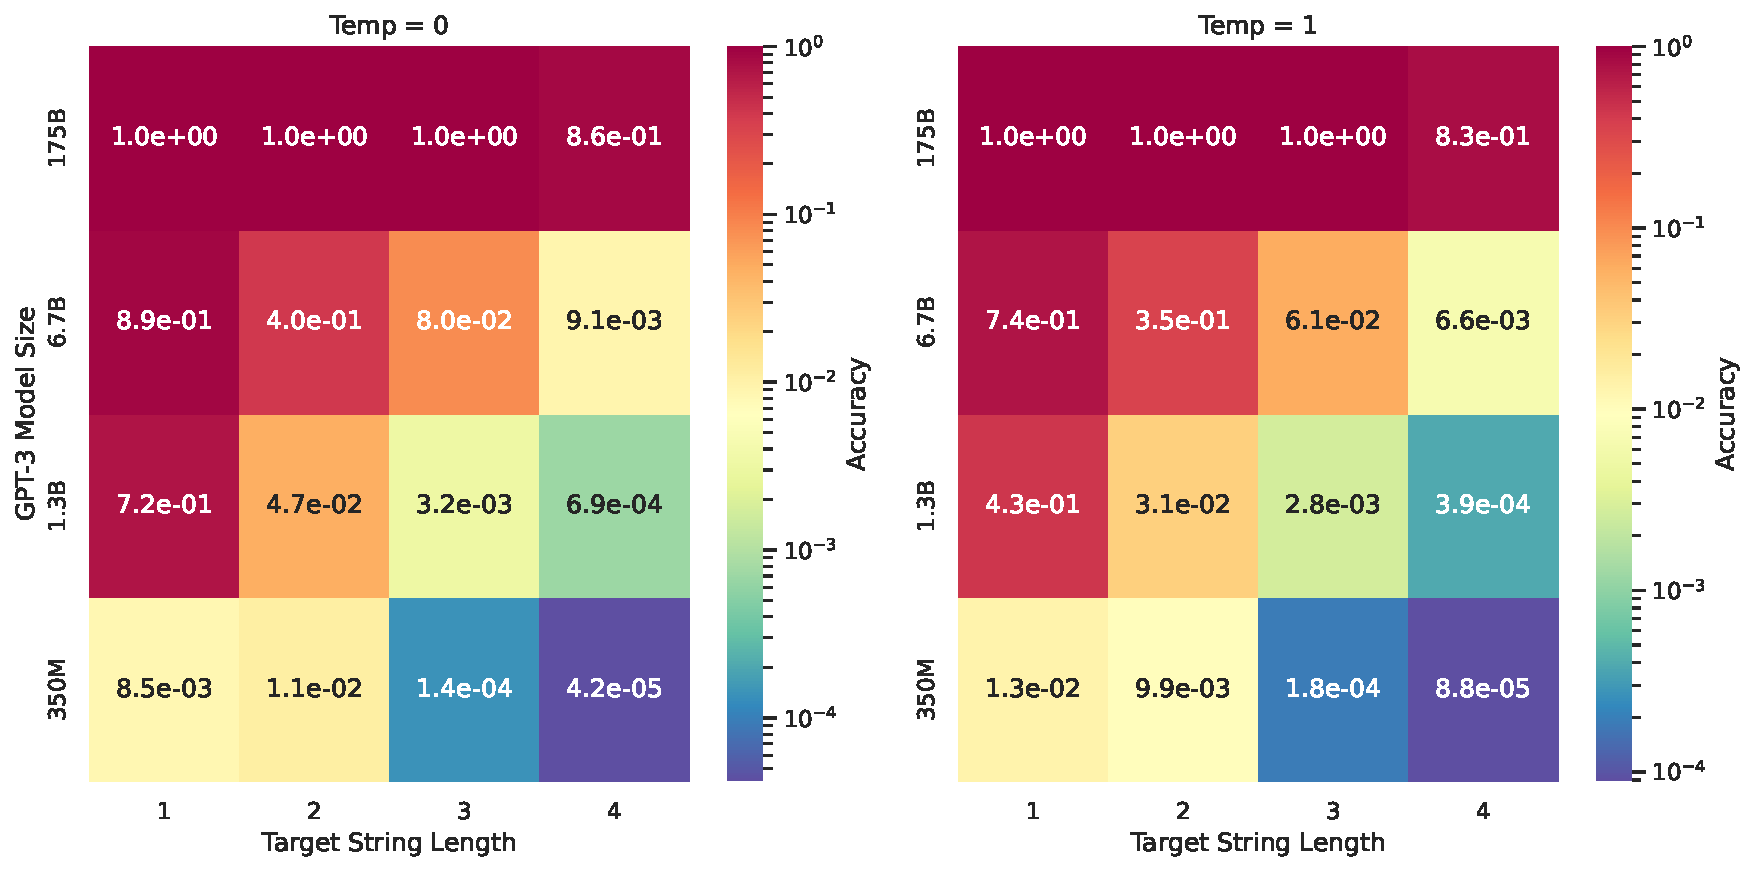
\includegraphics[width=0.95\textwidth]{figures/gpt3_integer_multiplication/heatmap_acc_by_model_size_by_target_str_len.pdf}
%     \end{minipage}
%     \caption{\textbf{}}
%     \label{fig:my_label}
% \end{figure}



\paragraph{Prediction: Emergent Abilities Disappear With Better Statistics}

We next tested our second prediction: that even on nonlinear metrics such as accuracy, smaller models do not have zero accuracy, but rather have non-zero above-chance accuracy \textit{commensurate with choosing to use accuracy as the metric}. In order to accurately measure models' accuracy, we increased the resolution by generating additional test data, and found that on both arithmetic tasks, all models in the InstructGPT/GPT-3 family achieve above-chance accuracy (Fig. \ref{fig:gpt_improve_resolution}). This confirms our second prediction. We also observe that as the target string length increases, the accuracy falls approximately geometrically with the length of the target string, confirming the second half of our third prediction. These results additionally demonstrate that the researcher's choice of metric has the effect that one should predict accuracy to have, i.e., geometric decay with the target length.

% \subsection{GPT-3's per-token probability of selecting the correct token}

% \begin{figure}
%     \centering
%     \begin{minipage}{.32\textwidth}
%         \centering
%         Mathematical Model
%         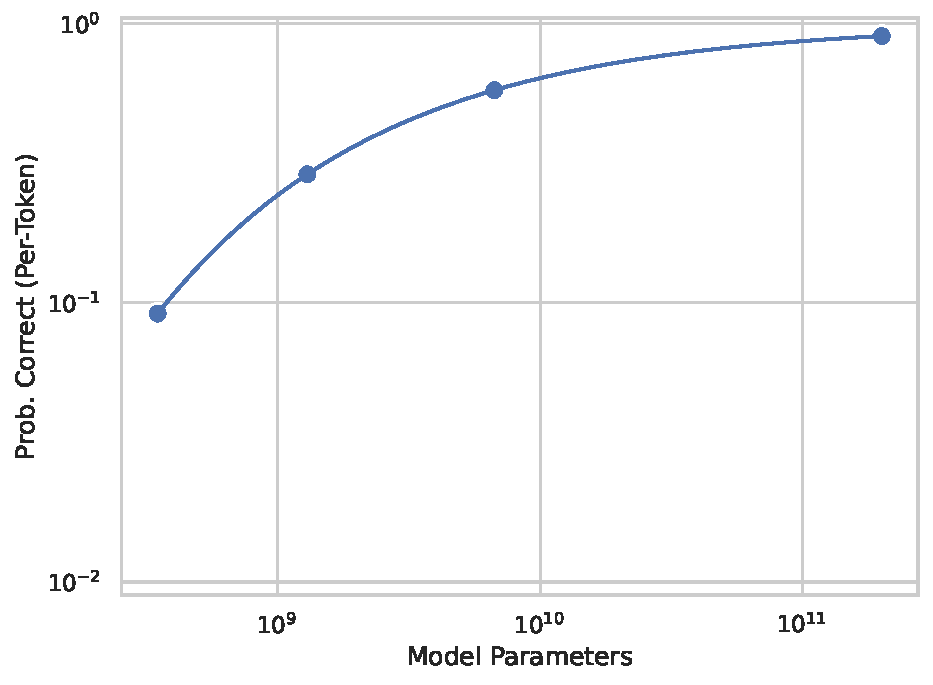
\includegraphics[width=0.95\textwidth]{figures/toy_emergence/prob_correct_per_token_vs_model_size.pdf}
%     \end{minipage}%
%     \begin{minipage}{0.32\textwidth}
%         \centering
%         4-Digit Integer Addition
%         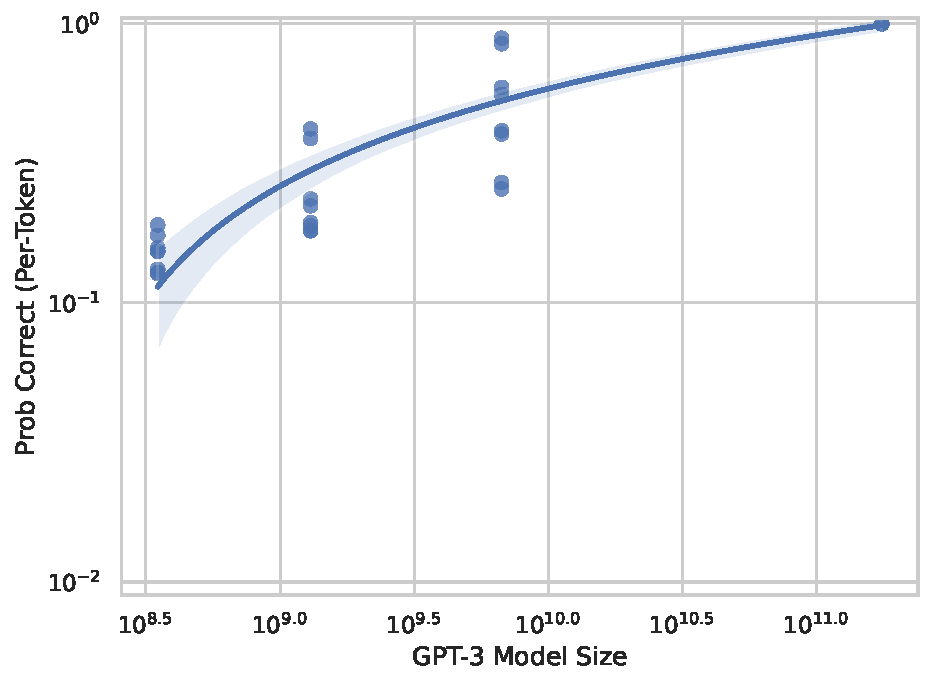
\includegraphics[width=0.95\textwidth]{figures/gpt3_integer_addition/prob_correct_per_token_vs_model_size.pdf}
%     \end{minipage}%
%     \begin{minipage}{0.35\textwidth}
%         \centering
%         2-Digit Integer Multiplication
%         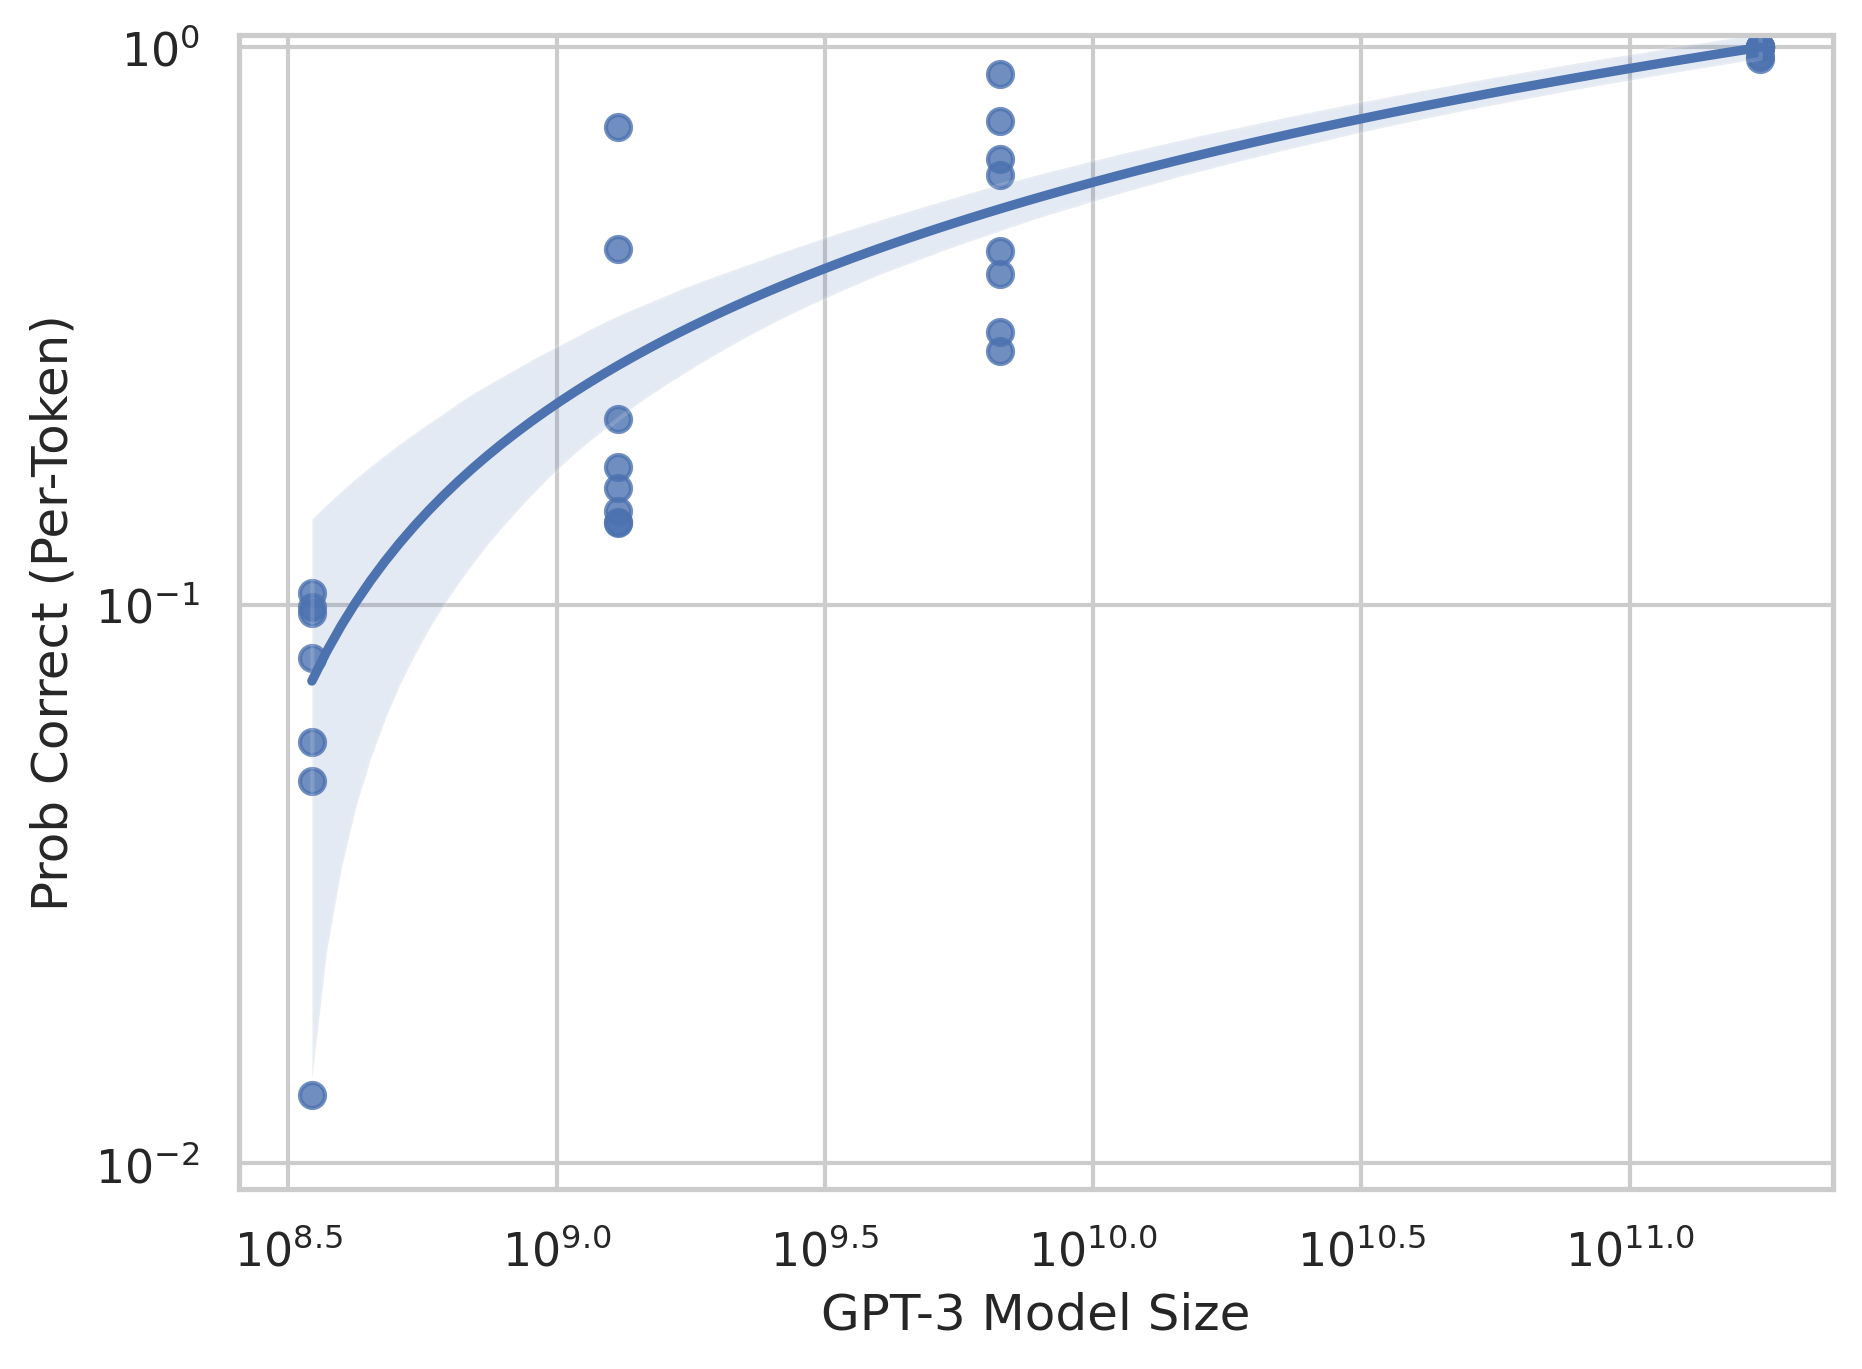
\includegraphics[width=0.95\textwidth]{figures/gpt3_integer_multiplication/prob_correct_per_token_vs_model_size.png}
%     \end{minipage}
%     \caption{Are these figures worth including? Unclear... Probably not}
%     \label{fig:my_label}
% \end{figure}

% As an additional test for our mathematical model, we can leverage the fact that the GPT-3 family follows a neural scaling law \cite{brown2020language} to compute the family's per-token probability of selecting the correct token in two different ways. In the first approach, we can invert the published test cross entropies to recover the per-token probability correct; in the second approach, we can take the model's output generated strings and compute the per-token probability correct.


\section{Meta-Analysis of Claimed Emergent Abilities}

Analyzing the GPT family is possible because the models are publicly queryable.
However, other model families claimed to exhibit emergent abilities are not publicly queryable, nor are their generated outputs publicly available, meaning we are limited to analyzing the published results themselves \cite{ganguli2022predictability, wei2022emergent, wei2022bigbench}.
Our alternative explanation makes two predictions.
\begin{enumerate}
    \item At the ``population level" of Task-Metric-Model Family triplets, emergent abilities should appear predominantly on specific \textit{metrics}, not \textit{task-model family} pairs, and specifically with nonlinear and/or discontinuous metrics.
    \item On individual Task-Metric-Model Family triplets that display an emergent ability, changing the metric to a linear and/or continuous metric should remove the emergent ability.
\end{enumerate}

% First, whether model families display emergent capabilities should be metric dependent, with sharp metrics being more likely to produce emergent abilities.
% Second, on task-metric-model family triplets that display emergence, considering less sharp metrics should display little-to-no emergence.
To test these predictions, we used to claimed emergent abilities on BIG-Bench \cite{srivastava2022beyond, wei2022emergent} due to the benchmark being pertinent and publicly available.

\paragraph{Prediction: Emergent Abilities Should Appear with Metrics, not Task-Model Families}

If emergent abilities are real, one should expect task-model family pairs to show emergence for all reasonable metrics. However, if our alternative explanation is correct, we should expect emergent abilities to appear only under certain metrics. To test this, we analyzed on which metrics emergent abilities appear. To determine whether a task-metric-model family triplet exhibits a possible emergent ability, we used a metric from previous work \cite{srivastava2022beyond}. Letting $y_i \in \mathbb{R}$ denote model performance at model scales $x_i \in \mathbb{R}$, sorted such that $x_i < x_{i+1}$, the emergence score is:
%
\begin{equation}
    \text{Emergence Score}\Big(\Big\{ (x_n, y_n) \Big\}_{n=1}^N \Big) \quad \defeq \quad \frac{\text{sign}(\arg \max_i y_i - \arg \min_i y_i)(\max_i y_i - \min_i y_i)}{\sqrt{\text{Median}(\{ (y_i - y_{i-1})^2 \}_i)}}
\end{equation}


\begin{figure}
    \centering
    \begin{minipage}[c]{0.7\textwidth}
     \centering
        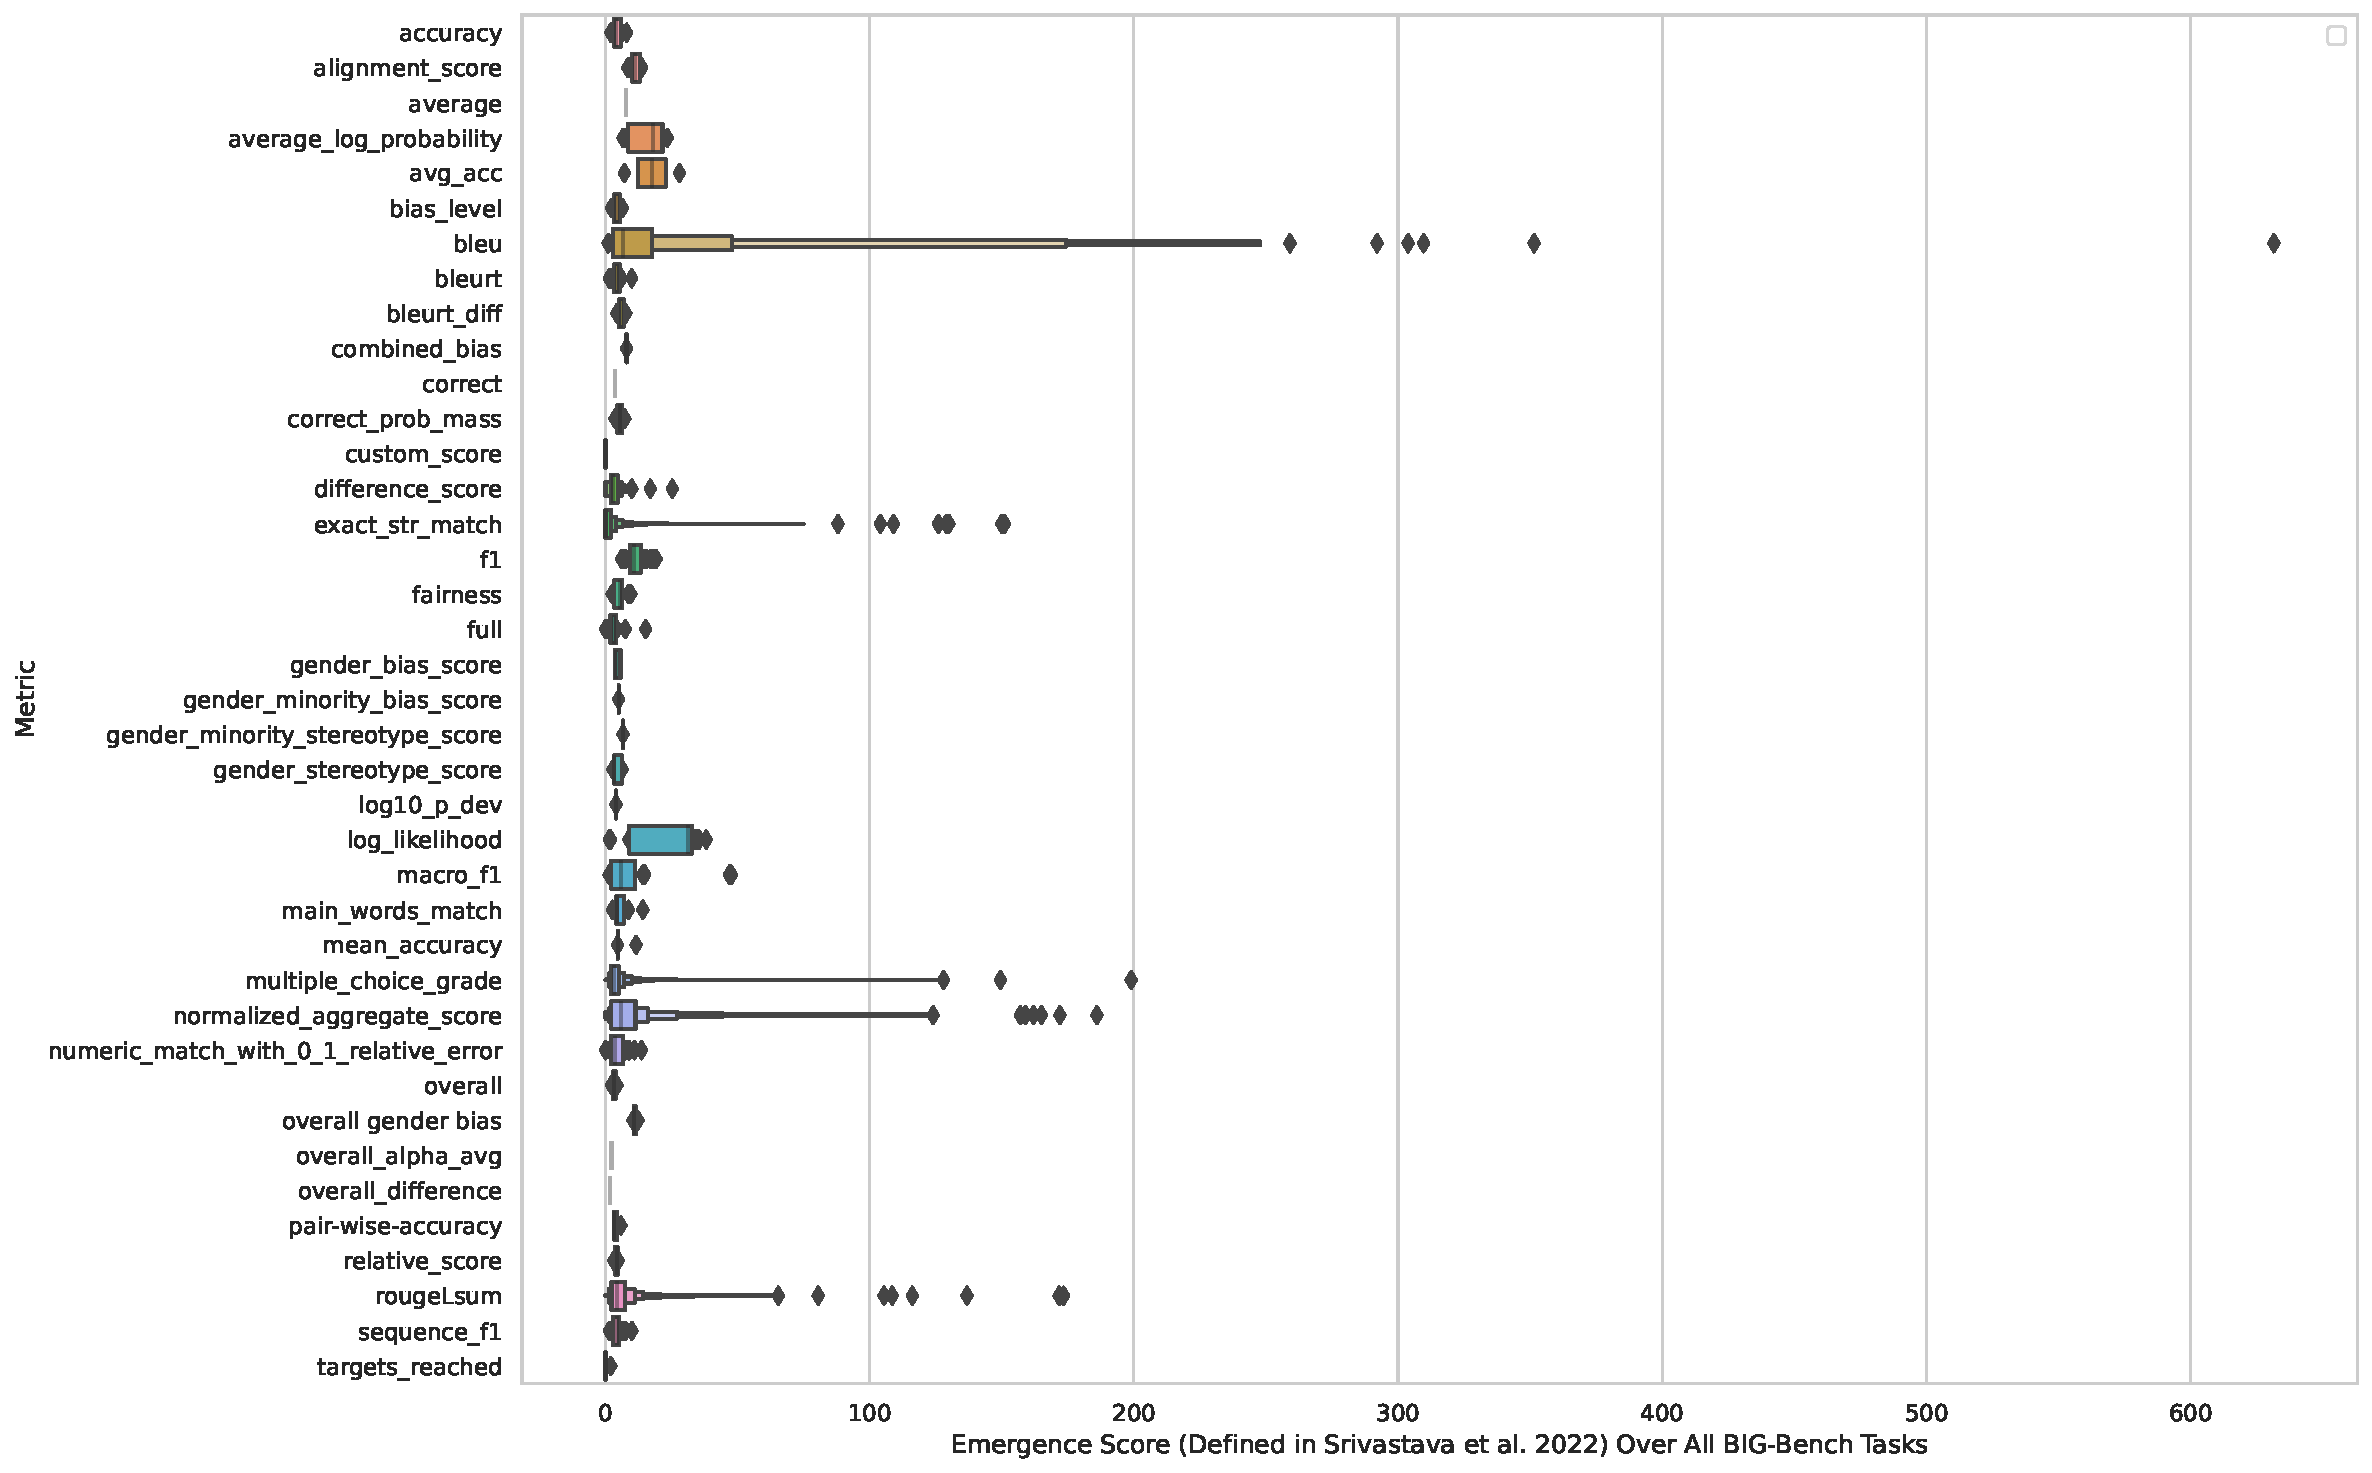
\includegraphics[width=0.95\textwidth]{figures/big_bench_emergent_tasks/big_bench_breakthrough_scores_by_metric.pdf}%
     \end{minipage}%
     \begin{minipage}[c]{0.3\textwidth}
     \centering
        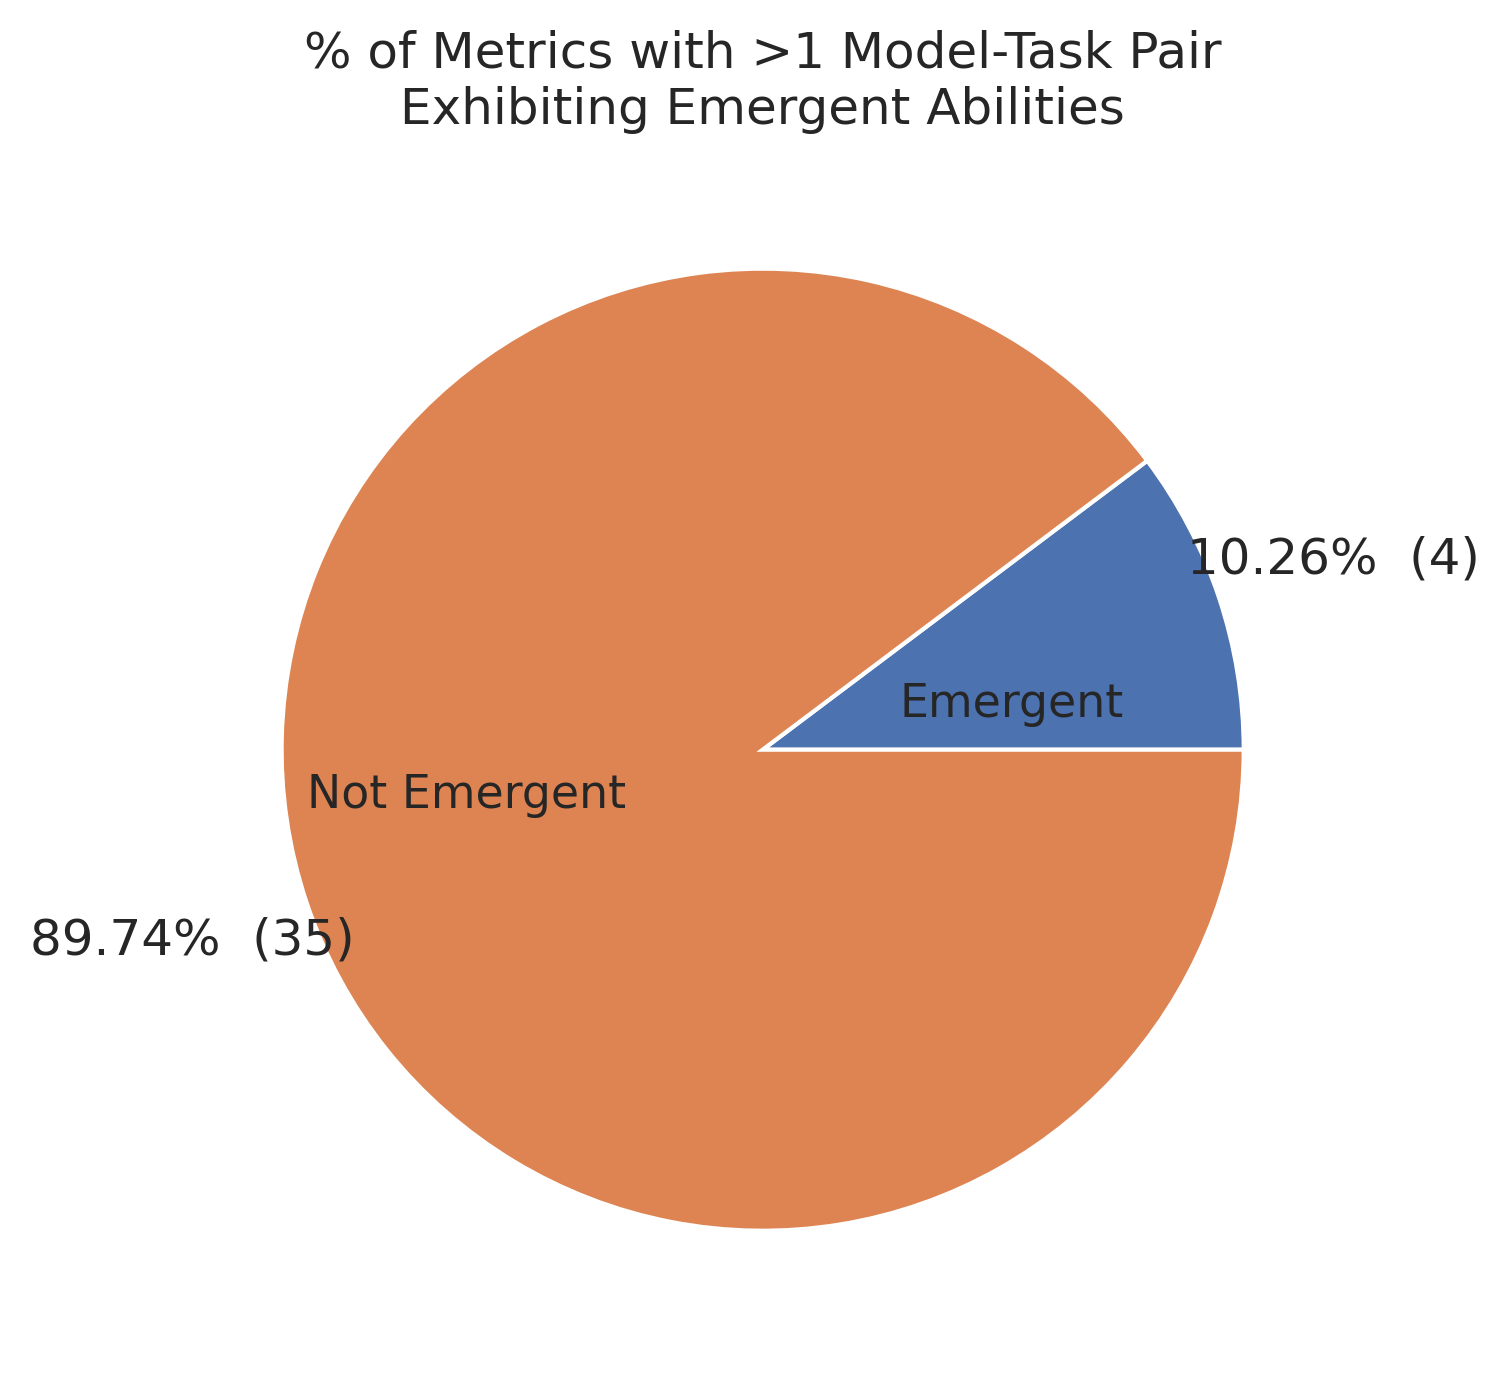
\includegraphics[width=0.85\textwidth]{figures/big_bench_emergent_tasks/emergence_percent_pie.png}
        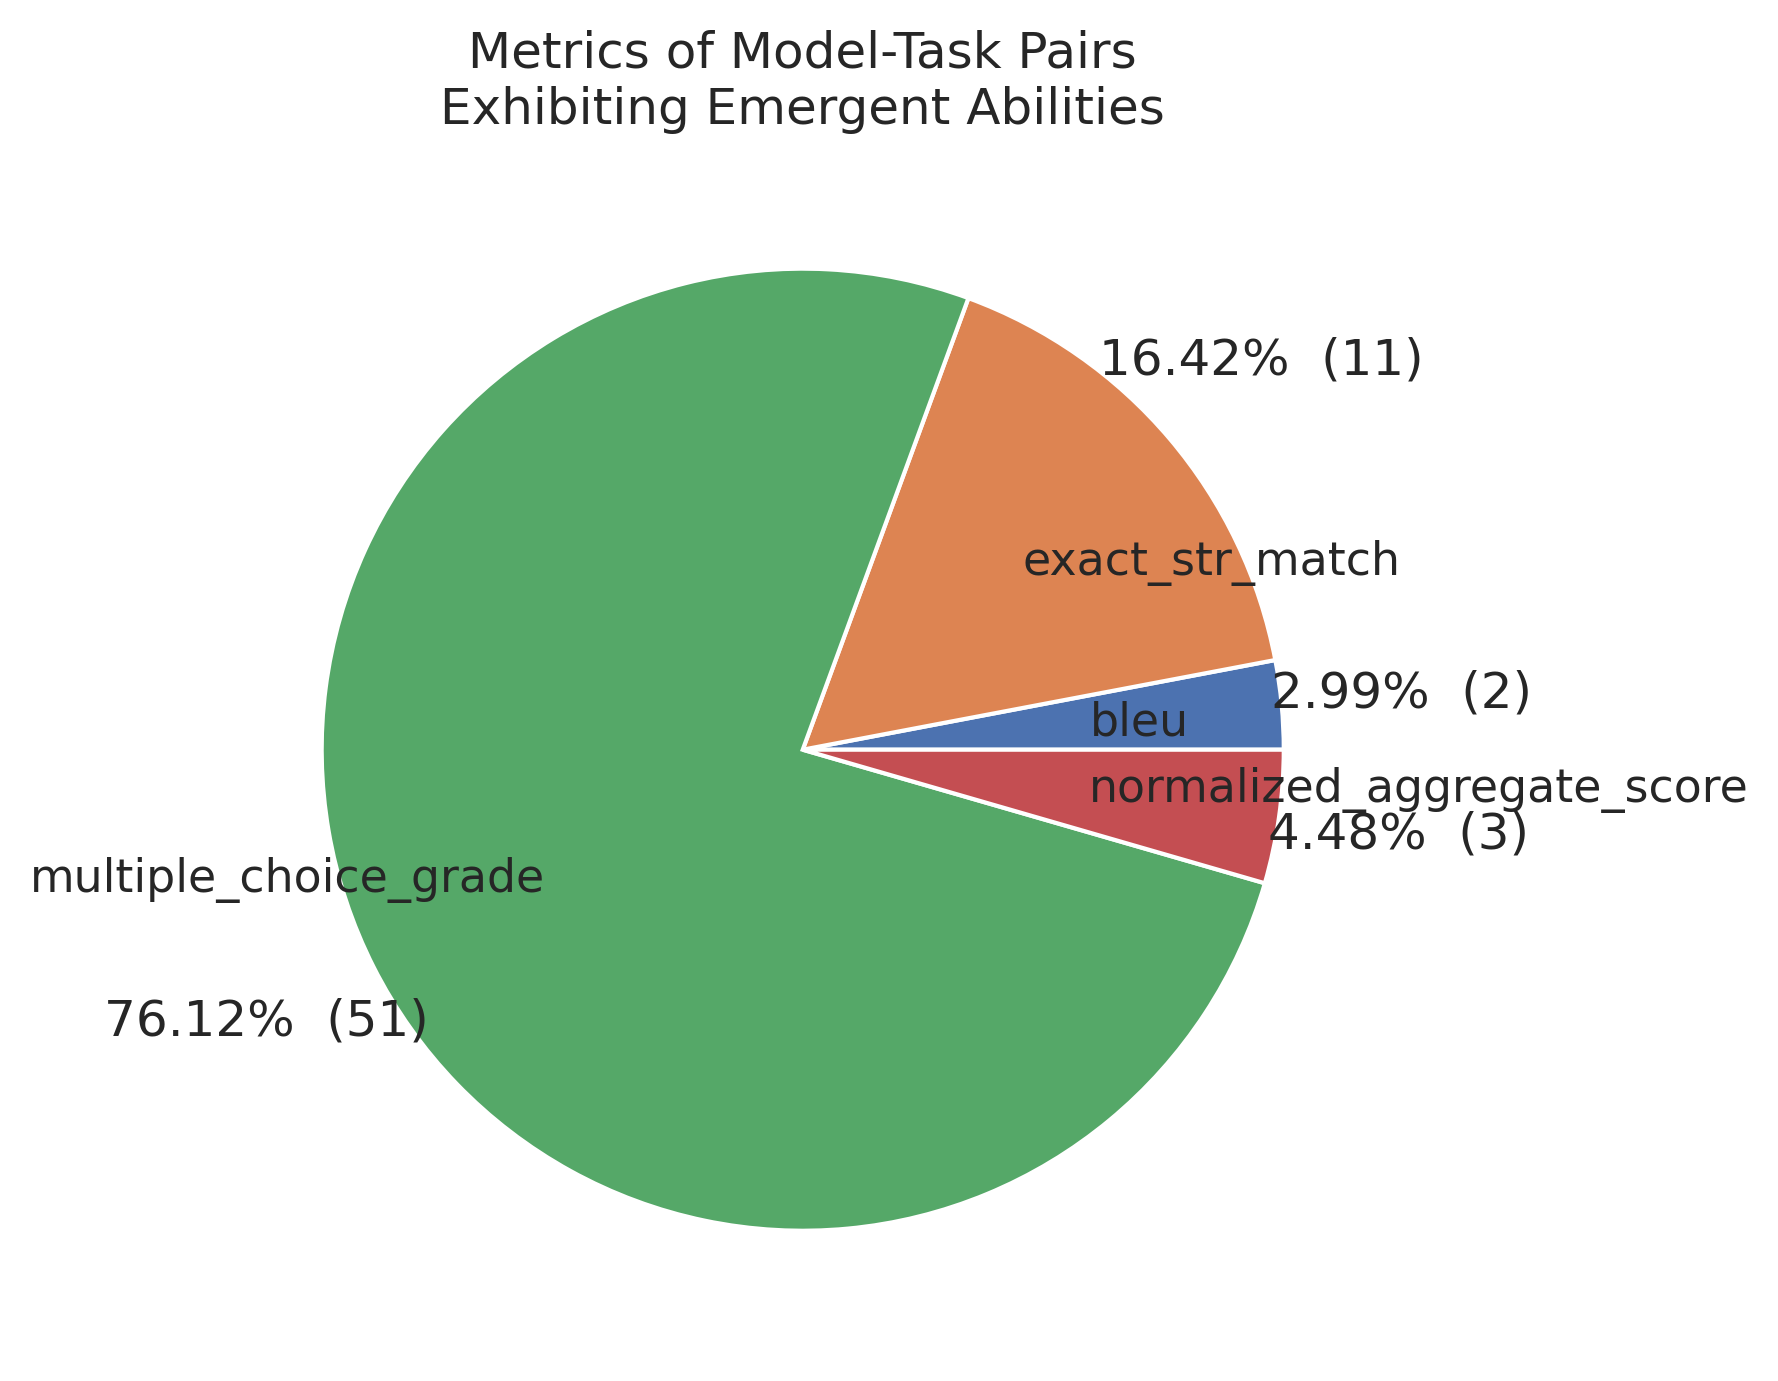
\includegraphics[width=0.95\textwidth]{figures/big_bench_emergent_tasks/metric_given_emergent_pie.png}
     \end{minipage}
    \caption{\textbf{Emergent abilities appear only for specific metrics, not task-model families.} (A) \textit{Possible} emergent abilities appear with \textit{at most} 5 out of 39 BIG-Bench metrics. (B) Hand-annotated data by \cite{wei2022bigbench} reveals emergent abilities appear only under 4 preferred metrics. (C) $>92\%$ of emergent abilities appear under one of two metrics: Multiple Choice Grade and Exact String Match.}
    \label{fig:big_bench_breakthrough_scores_by_metric}
\end{figure}

We found that most metrics used in BIG-Bench have \textit{zero} task-model family pairs that exhibit emergent abilities: of the 39 preferred metrics in BIG-Bench, at most 5 display emergence (Fig. \ref{fig:big_bench_breakthrough_scores_by_metric}A). Many of the 5 are nonlinear and/or discontinuous, e.g., Exact String Match, Multiple Choice Grade, ROUGE-L-Sum (App. \ref{app:metric_scaling:rougeLsum}). Notably, because BIG-Bench often scores models on tasks using multiple metrics, the \textit{lack} of emergent abilities under other metrics suggests that emergent abilities do not appear when model outputs are scored using other metrics.

Because emergence score only \textit{suggests} emergence, we also analyzed hand-annotated task-metric-model family triplets \cite{wei2022bigbench}, which revealed emergent abilities appear with $4 / 39$ metrics (Fig. \ref{fig:big_bench_breakthrough_scores_by_metric}B), and 2 metrics account for $>92\%$ of claimed emergent abilities (Fig. \ref{fig:big_bench_breakthrough_scores_by_metric}C): Multiple Choice Grade and Exact String Match. Multiple Choice Grade is discontinuous, and Exact String Match is nonlinear.


 \begin{figure}
    \centering
    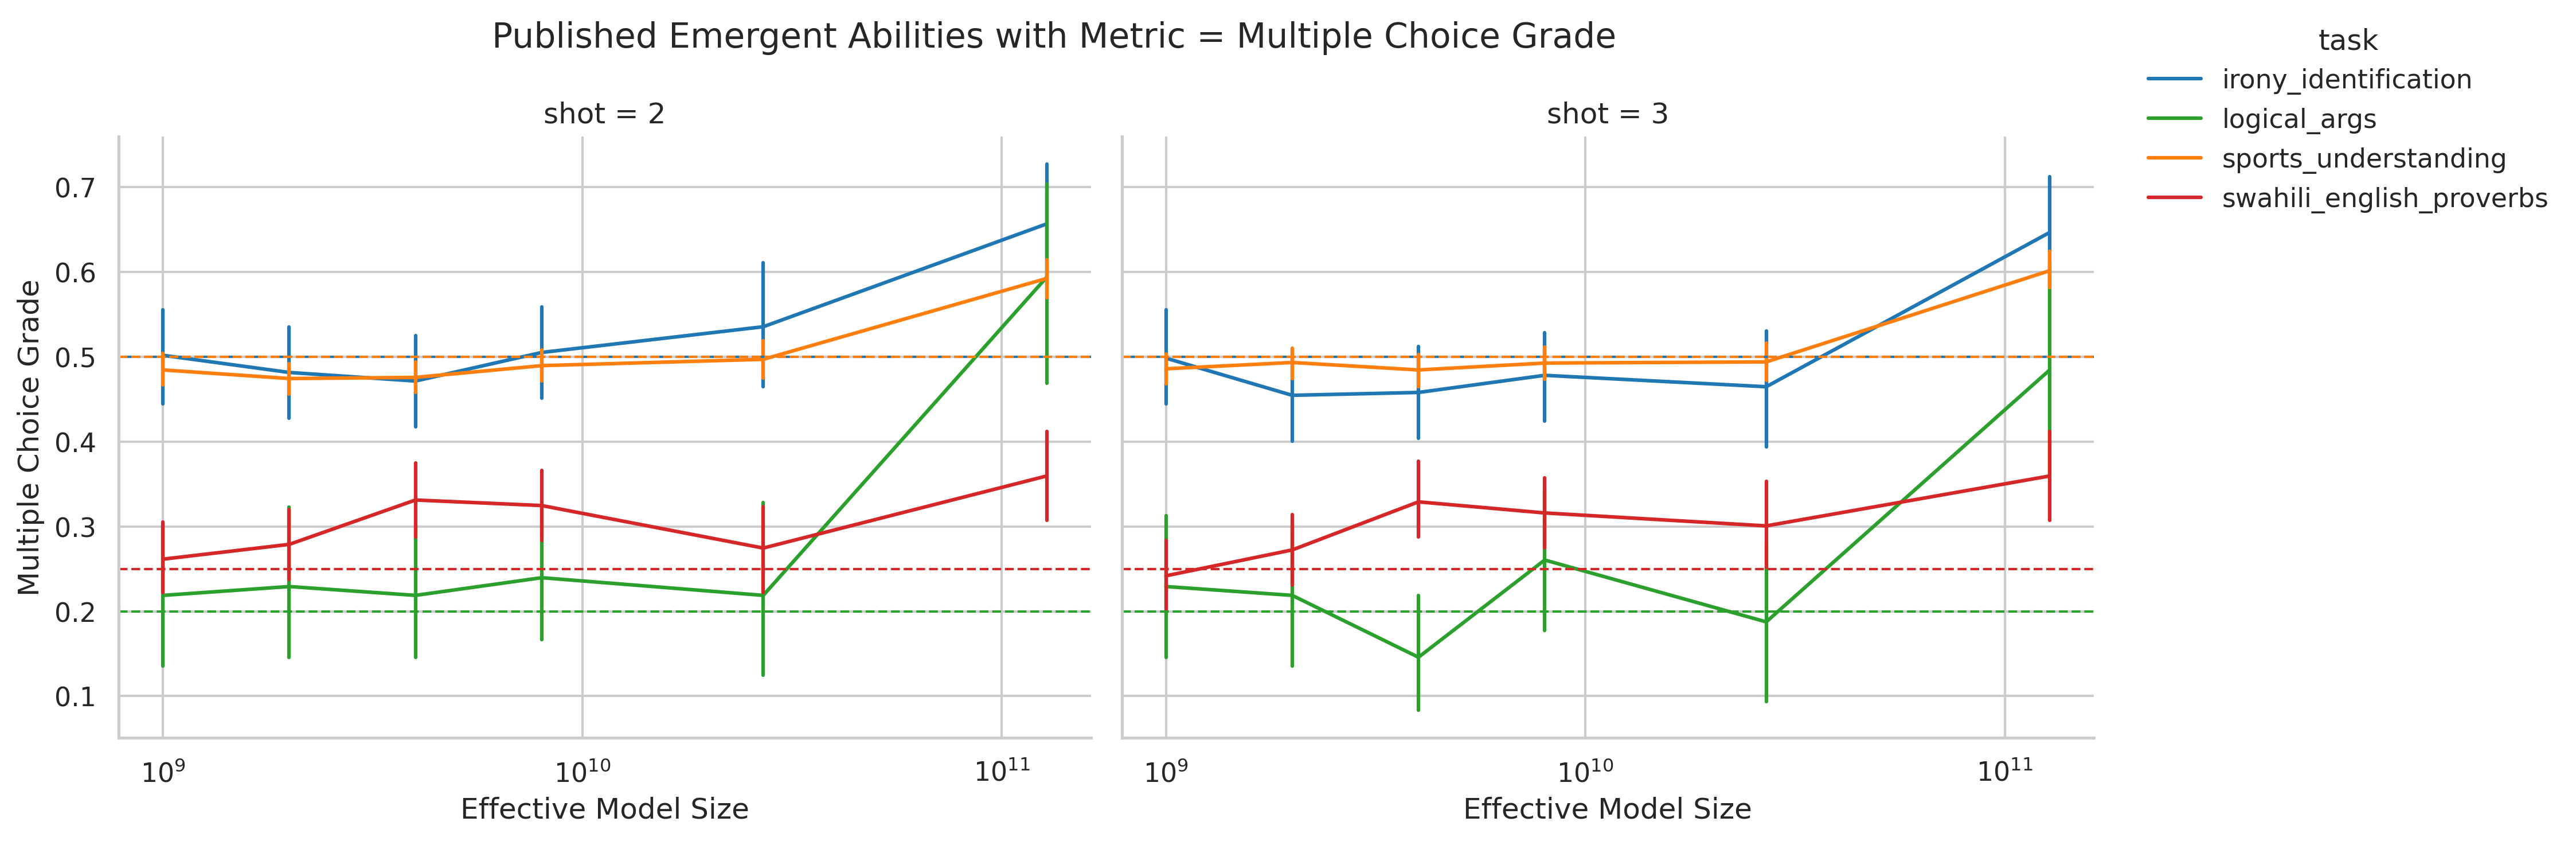
\includegraphics[width=0.49\textwidth]{figures/big_bench_emergent_tasks/score_vs_model_size_by_task_split_shot_other_metric=multiple_choice_grade.png}%
    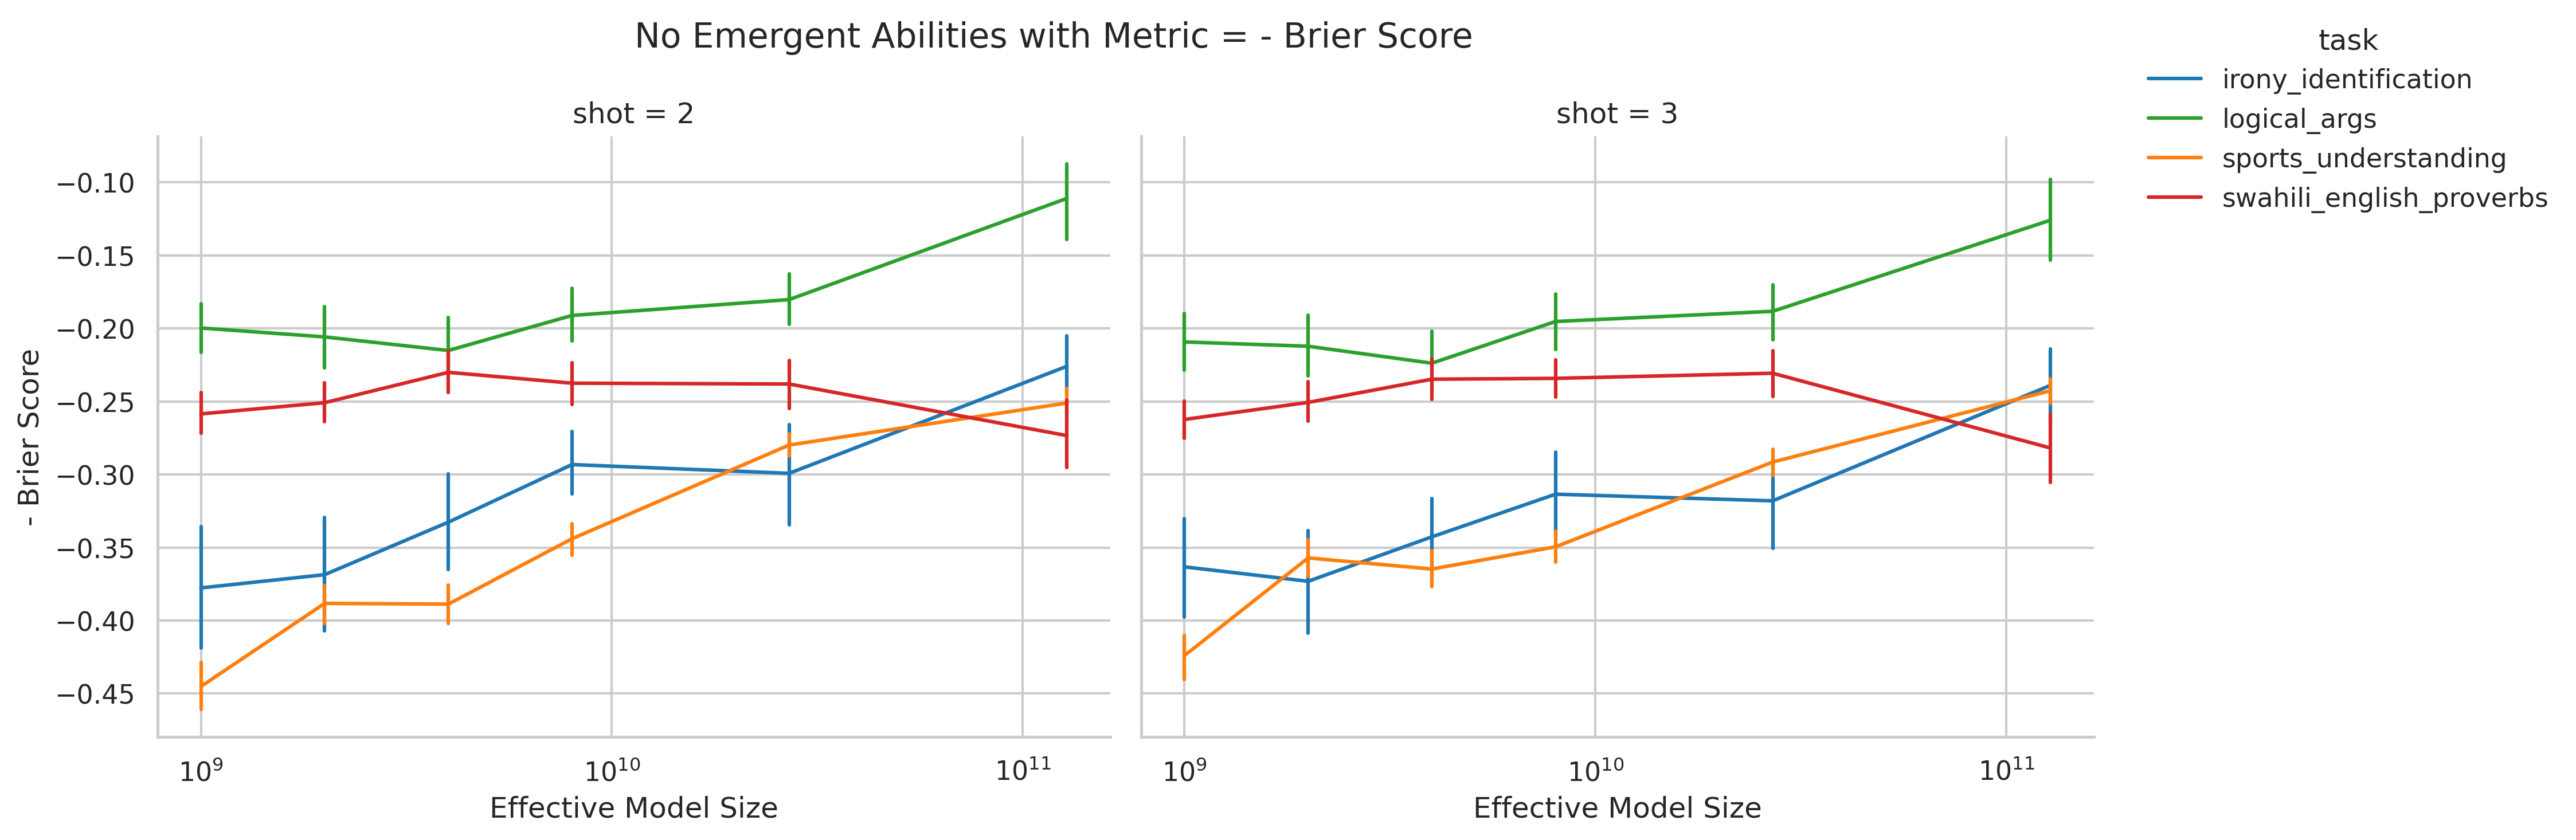
\includegraphics[width=0.49\textwidth]{figures/big_bench_emergent_tasks/score_vs_model_size_by_task_split_shot_other_metric=calibration_multiple_choice_brier_score.png}
    \caption{\textbf{Changing the metric when evaluating task-model family pairs causes emergent abilities to disappear.} Left: The LaMDA model family displays emergent abilities when measured under the discontinuous Multiple Choice Grade. Right: The LaMDA model family's emergent abilities disappear when measured under a continuous BIG-Bench metric: Brier Score.}
    \label{fig:big_bench_brier_score}
\end{figure}

\paragraph{Prediction: Changing Metric Removes Emergent Abilities}

% \footnote{BIG-Bench contains LaMDA models of sizes 16M, 53M, 125M, 244M, 422M.}
To test our second prediction, 
%we analyzed hand-annotated emergent abilities of \cite{wei2022bigbench}. 
we focused on the LaMDA family \cite{thoppilan2022lamda} because its outputs are available through BIG-Bench.
% whereas other model families' outputs are not.
%The smallest published LaMDA model has 2B parameters, but many LaMDA models in BIG-Bench are significantly smaller and we were unable to identify the sources of these smaller models, so we excluded them.
% according to \cite{wei2022bigbench}
For our analysis, we identified tasks on which LaMDA displays emergent abilities with Multiple Choice Grade, then asked whether LaMDA still displays emergent abilities on the same tasks with a different BIG-Bench metric: Brier Score \cite{brier1950verification}. 
Brier Score is a strictly proper scoring rule for predictions of mutually exclusive outcomes; for a binary outcome, the Brier Score simplifies to the mean squared error between the outcome and its predicted probability mass.
LaMDA's emergent abilities on the discontinuous Multiple Choice Grade disappeared when we changed the metric to the continuous Brier Score (Fig. \ref{fig:big_bench_brier_score}).
%This further supports our alternative explanation that emergent abilities are induced by the researcher's chosen metric.
These results support our alternative explanation that emergent abilities are induced by the chosen metric.
%, not unpredictable changes in the model family on a specific task with scale.
\section{Inducing Emergent Abilities in Networks on Vision Tasks}
\label{sec:inducing_emergence_vision}

To demonstrate how emergent abilities can be induced by the researcher's choice of metric, we show how to produce emergent abilities in deep networks of various architectures: fully connected, convolutional, self-attentional.
We focus on vision tasks because abrupt transitions in vision models' capabilities have not been observed to the best of our knowledge; this is one reason why emergence in large language models is considered so interesting.
% Second, some vision tasks can be solved by modestly sized networks and therefore can enable us to construct entire model families with scales spanning multiple orders of magnitude.
% We specifically use simple networks on well-studied tasks to drive home the point that there is nothing new here.
For the convolutional example, see App. \ref{app:sec:inducing_emergence_vision}.

\paragraph{Emergent Reconstruction of CIFAR100 Natural Images by Nonlinear Autoencoders}

\begin{figure}
    \centering
    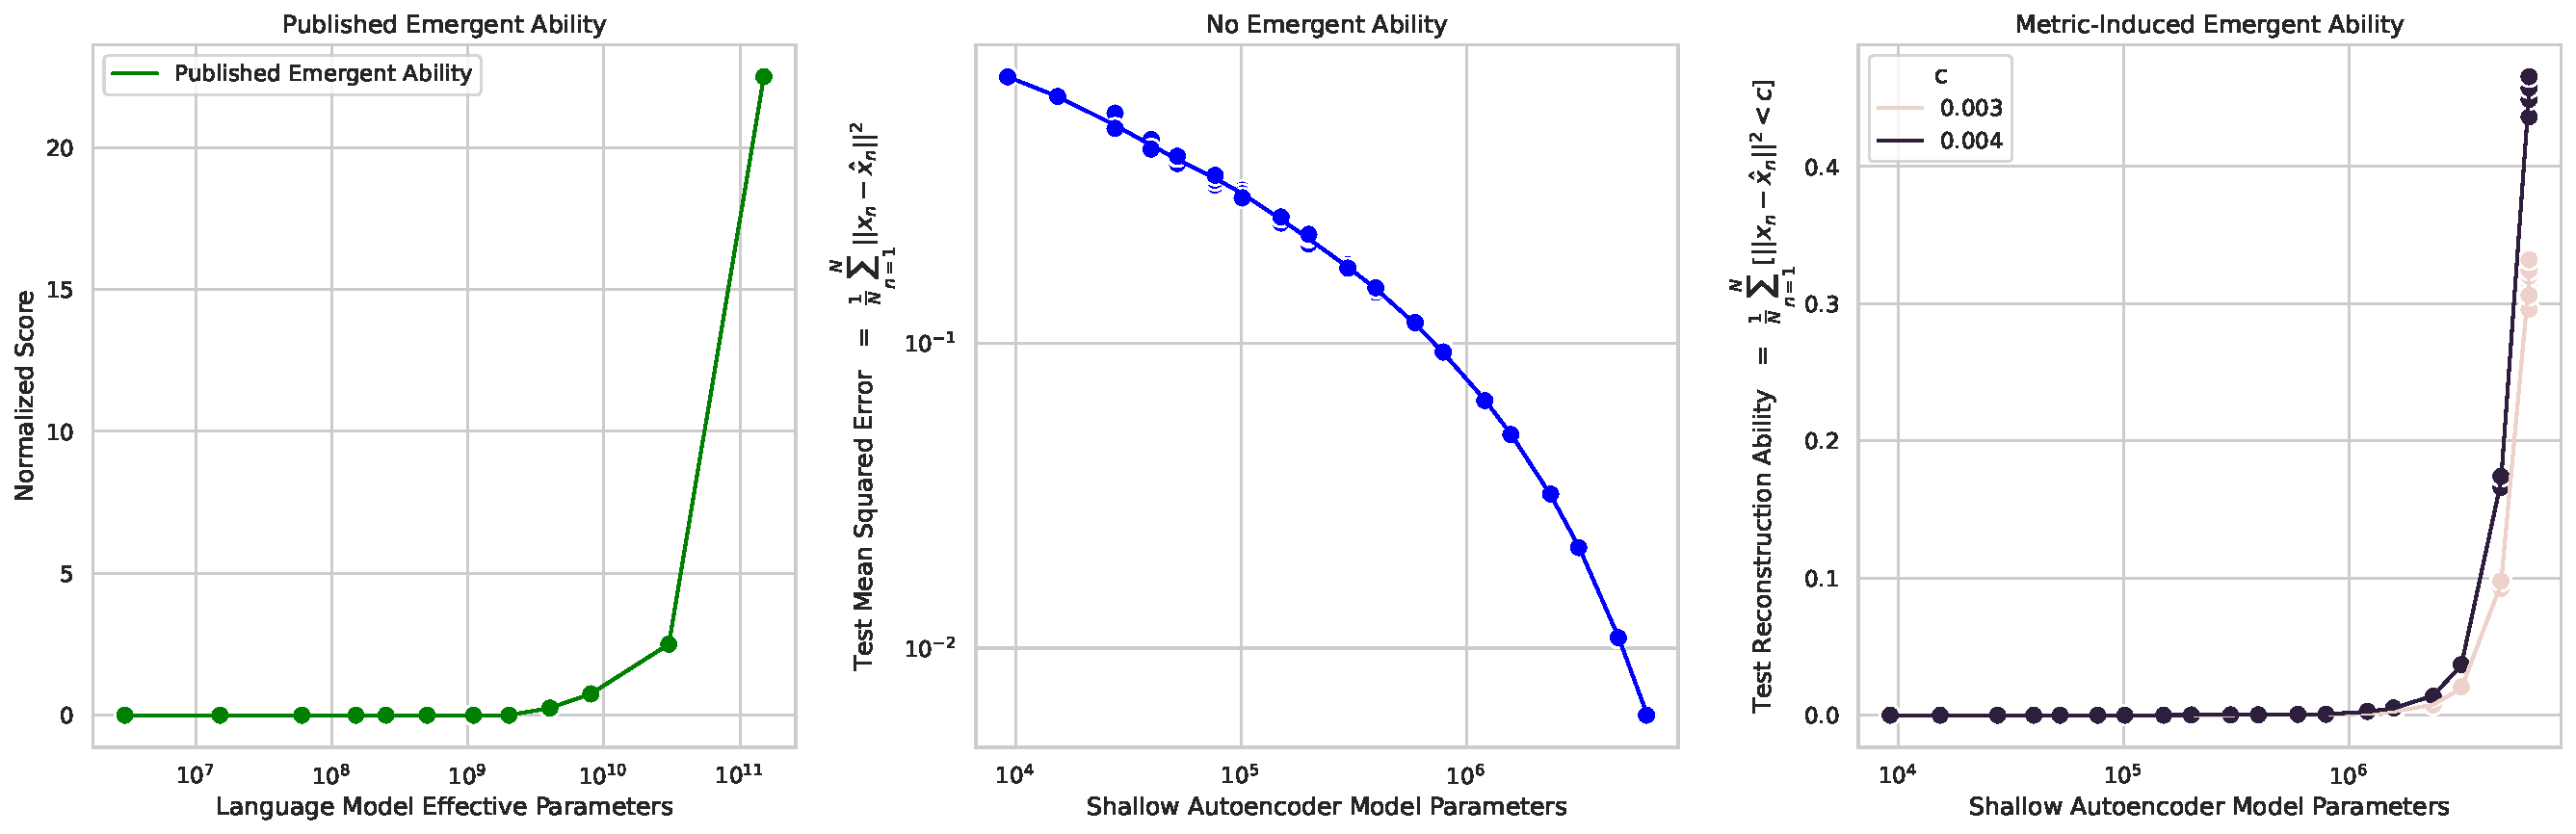
\includegraphics[width=0.9\textwidth]{figures/vision/no_emergence_and_emergence_dataset=cifar100.pdf}
    \caption{\textbf{Induced emergent reconstruction ability in shallow nonlinear autoencoders.} (A) A published emergent ability at the BIG-Bench Periodic Elements task \cite{srivastava2022beyond}. (B) Shallow nonlinear autoencoders trained on CIFAR100 \cite{krizhevsky09learningmultiple} display smoothly decreasing mean squared reconstruction error. (C) Using a newly defined Reconstruction$_c$ metric (Eqn. \ref{eq:reconstruction}) induces an unpredictable change.}
    \label{fig:vision_cifar100}
\end{figure}

We first induce an emergent ability to reconstruct images in shallow (i.e., single hidden layer) nonlinear autoencoders trained on CIFAR100 natural images \cite{krizhevsky09learningmultiple}.
To emphasize that the sharpness of the metric is responsible for emergent abilities, and to show that sharpness extends to metrics beyond Accuracy, we intentionally define a discontinuous metric that measures a network's ability to reconstruct a dataset as the average number of test data with squared reconstruction error below threshold $c$:
%
\begin{equation}
    \text{Reconstruction}_c \Big(\{x_n \}_{n=1}^N \Big) \; \defeq \;
    \frac{1}{N} \sum_n \mathbb{I} \Big[ ||x_n - \hat{x}_n||^2 < c \Big]
    \label{eq:reconstruction}
\end{equation}
where $\mathbb{I}(\cdot)$ denotes an indicator variable and $\hat{x}_n$ is the autoencoder's reconstruction of $x_n$.
The autoencoder family displays smoothly decreasing squared reconstruction error as the number of bottleneck units increases (Fig. \ref{fig:vision_cifar100}B). Under our newly defined Reconstruction$_c$ metric and for particular choices of $c$, the autoencoder family exhibits a sharp and seemingly unpredictable image reconstruction ability (Fig. \ref{fig:vision_cifar100}C) that qualitatively matches published emergent abilities (Fig. \ref{fig:vision_cifar100}A).
% , for the BIG-Bench Periodic Elements task 

\paragraph{Emergent Classification of Omniglot Characters by Autoregressive Transformers}

\begin{figure}
    \centering
    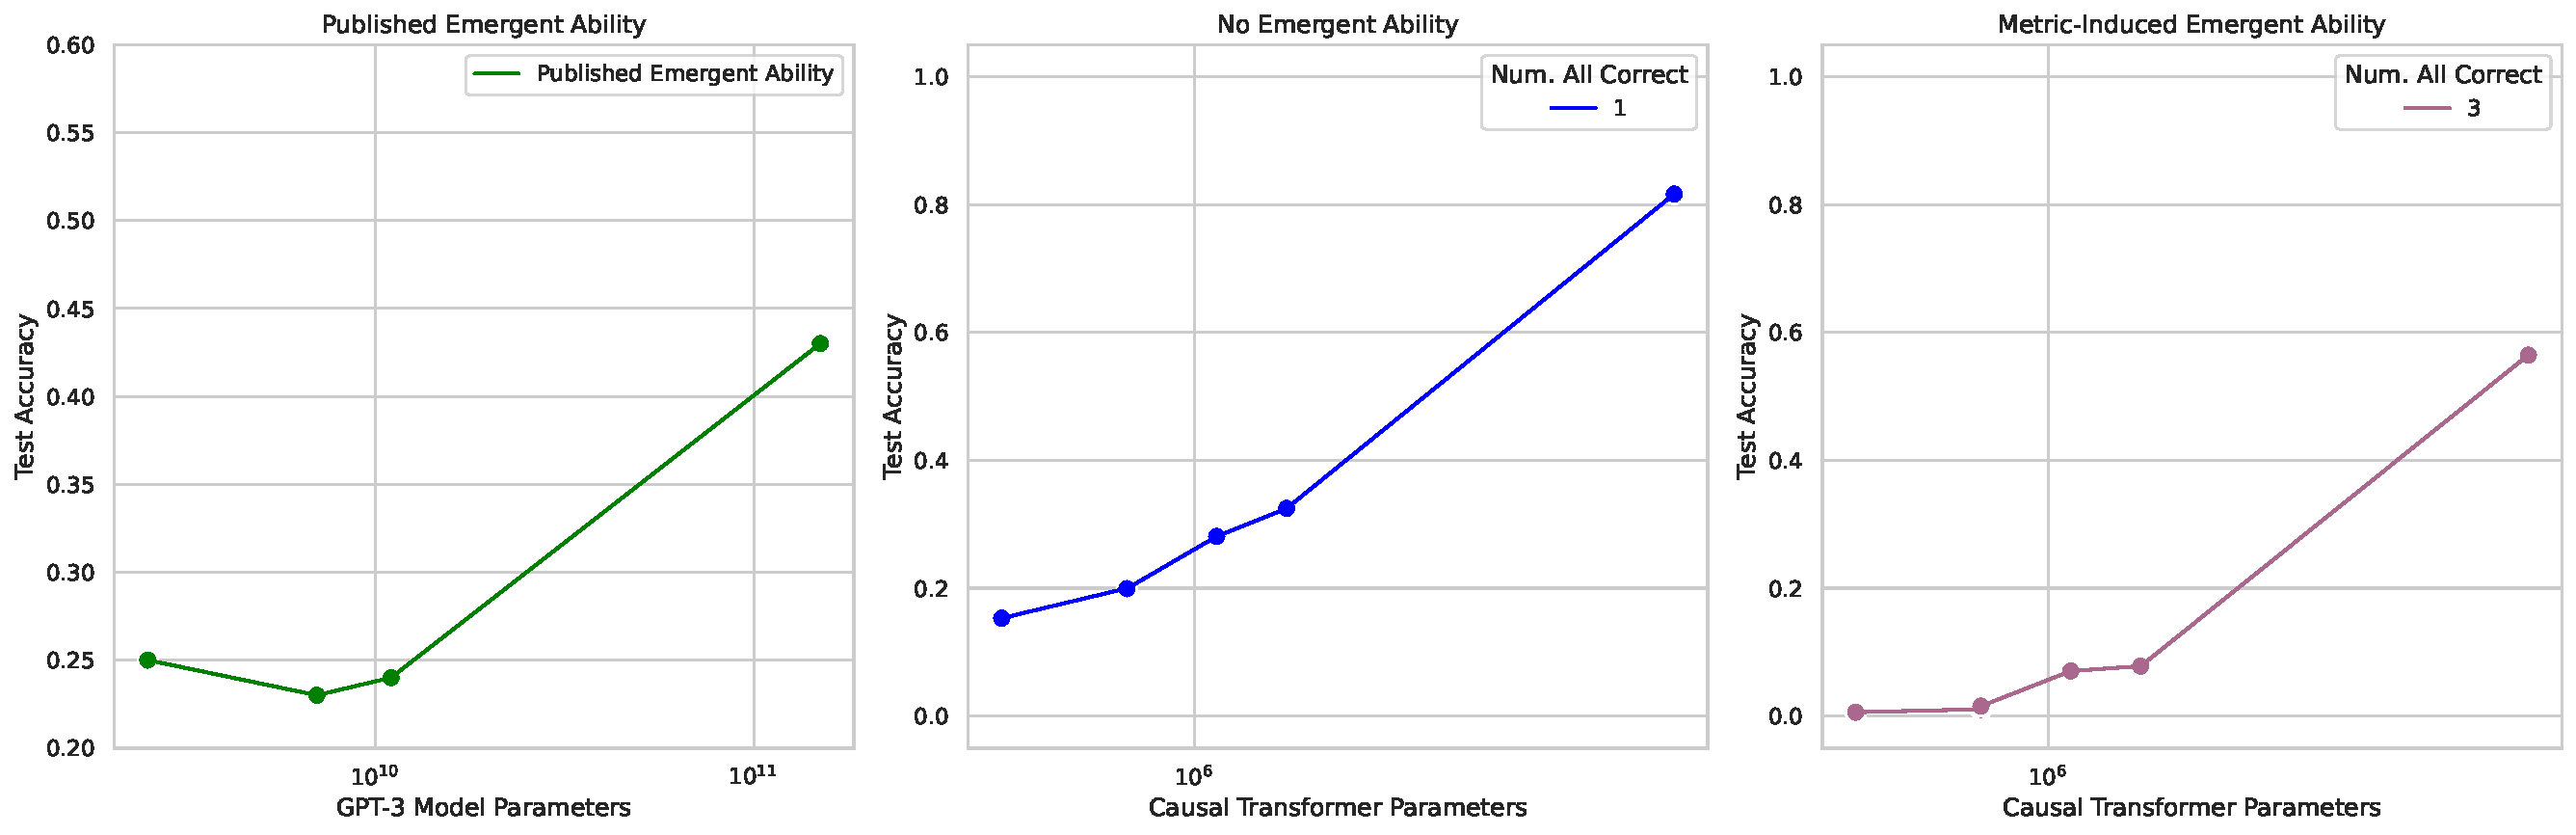
\includegraphics[width=0.9\textwidth]{figures/vision/no_emergence_and_emergence_dataset=omniglot.pdf}
    \caption{\textbf{Induced emergent classification ability in autoregressive Transformers.} (A) A published emergent ability on the MMLU benchmark \cite{ganguli2022predictability}. (B) Autoregressive transformers trained to classify Omniglot images display increasing accuracy with increasing scale. (C) When accuracy is redefined as classifying \textit{all} images correctly, a seemingly emergent ability appears.}
    \label{fig:vision_omniglot}
\end{figure}

We next induce emergent abilities in Transformers \cite{vaswani2017attention} trained to autoregressively classify Omniglot handwritten characters \cite{lake2015human}, in a setup inspired by recent work \cite{chan2022data}: Omniglot images are embedded by convolutional layers, then sequences of embedded image-image class label pairs are fed into decoder-only transformers.
We measure image classification performance on sequences of length $L \in [1, 5]$, again via \textit{subset accuracy}: $1$ if all $L$ images are classified correctly (Fig. \ref{fig:vision_omniglot}B), 0 otherwise.
Causal transformers display a seemingly emergent ability to correctly classify Omniglot handwritten characters (Fig. \ref{fig:vision_omniglot}C) that qualitatively matches published emergent abilities (Fig. \ref{fig:vision_omniglot}A).

% , e.g., Massive Multitask Language Understanding \cite{ganguli2022predictability}

\section{Related Work}

Srivastava et al. \cite{srivastava2022beyond} observed that while accuracy at a particular task can empirically appear sharp and unpredictable, cross entropy does not; the authors then hypothesized that emergent abilities may be partially attributed to the metric.
%writing: ``[Emergent abilities frequently appear] on tasks that have brittle or narrow metrics for success, emphasizing the importance of engineering graded metrics that can capture subthreshold improvements. Our results suggest that breakthrough performance can also occur on tasks that involve multistep reasoning. One possible explanation for the breakthrough phenomenon on multistep tasks is that the probability of success on the task scales like the product of the success probabilities on each step.”
Our paper converts their discussion into precise predictions, then quantitatively tests the predictions to reveal that: metric choice is likely wholly responsible for emergent abilities; well-known and widely-used metrics (including ones already used by \cite{srivastava2022beyond}) capture graded improvements; emergent abilities do not appear only for tasks involving multiple steps, and indeed appear most commonly on the discontinuous Multiple Choice Grade; metric choice can be used to induce emergent abilities in a novel domain (vision) in diverse architectures and tasks.

Caballero et al. \cite{caballero2022broken} explain emergence by assuming a piece-wise power law functional form; under this view, emergent abilities are real, caused by a change in the governing power law. In contrast, our work suggests that emergent abilities are induced by the researcher, even under a single power law. Michaud et al. \cite{michaud2023quantization} posit that emergent abilities may be real under strong data assumptions.

\section{Discussion}

Our paper presents an alternative explanation for claimed emergent abilities of large language models. For a fixed task and a fixed model family, the researcher can choose a metric to create an emergent ability or choose a metric to ablate an emergent ability. Ergo, \textit{emergent abilities may be creations of the researcher's choices, not a fundamental property of the model family on the specific task.} We emphasize that nothing in this paper should be interpreted as claiming that large language models \textit{cannot} display emergent abilities; rather, our message is that previously claimed emergent abilities in \cite{brown2020language, ganguli2022predictability,srivastava2022beyond,wei2022emergent} might likely be a mirage induced by researcher analyses.

Our paper has several implications. Firstly, a task and a metric are distinct and meaningful choices when constructing a benchmark. Secondly, when choosing metric(s), one should consider the metric's effect on the per-token error rate and adapt their measuring process accordingly, e.g., if one chooses accuracy, one should make sure to have sufficient data to accurately measure accuracy to avoid the risk of drawing invalid scientific conclusions.
%Thirdly, what metrics \textit{should} one choose? If the goal is to measure how useful a model's outputs are to humans, then harsh metrics like Accuracy or Multiple Choice Grade may diverge from human preferences.
%For instance, suppose that Model A places 5\% probability mass on a Yes/No question's correct answer, and Model B places 40\% probability mass on the correct answer; under Multiple Choice Grade, these two models score equivalently: 0. To offer one real-world anecdote, while learning how to use BIG-Bench, the authors accidentally discovered within BIG-Bench a question ``Q: What is 4 plus 5?" and a model's answer ``The sum of 4 and 5 is 9" that was scored as 0 because regex is used to extract the first occurring integer.
%Consequently, determining to what extent common NLP metrics correlate with human preferences should be a priority to avoid overfitting to NLP metrics.
Thirdly, when making claims about capabilities of large models, including proper controls is critical. In this particular setting, emergent abilities claims are possibly infected by a failure to control for multiple comparisons. In BIG-Bench alone, there are $\geq$ 220 tasks, $\sim 40$ metrics per task, $\sim10$ model families, for a total of $\sim 10^6$ task-metric-model family triplets, meaning probability that \textit{no} task-metric-model family triplet exhibits an emergent ability by random chance  might be small.
Fourthly, scientific progress can be hampered when models and their outputs are not made public for independent scientific investigation.

% TODO: Decide whether to keep this or move to appendix. Our findings reveal that metrics exhibiting apparent emergence disproportionately penalize smaller-scale models. 
% Monitoring alternative metrics unveil consistent, predictable alterations as the model scales. 
% Consequently, small-scale experimentation remains valuable, provided appropriate metrics are employed to avoid undue penalization. 
% Specifically, GPT-4 development incorporated small-scaling experimentation alongside scaling laws [1].


% Commented out for NeurIPS

% \section{Contributions}

% RS conceived of the research direction, collected data, ran experiments and analyzed results. SK supervised and guided the project. BM also provided guidance.

% \section{Acknowledgements}

% We thank our colleagues Max Lamparth, Mikail Khona, Kateryna Pistunova, Victor Lecomte, and Zane Durante for discussing our findings with us and providing much appreciated feedback.


\clearpage
% \bibliographystyle{plainnat}
\bibliographystyle{plain}
\bibliography{references}

\clearpage
\section{Implementation}
\label{app:implementation}

% Sampling from a cascade consists of 

\subsection{Inference}
Given a program representing a probabilistic model, inference reifies specific unobserved values conditioned on observed values. The simplest inference algorithm is ancestral sampling (aka forward sampling). The basic inference API is:

\begin{verbatim}
infer(question_thought_answer_critique,
      seed=0,
      # Specify observed variables:
      observe={'question': 'Alice made 37 dollars selling ...',
               'critique': 'The reasoning and arithmetic are correct.'},
      # Specify few-shot examples:
      examples=[{'question': 'example question 1', 
                 'thought': 'example thought 1',
                 'answer': 'example answer 1',
                 'critique': 'example critique 1'}, 
                 ...])
\end{verbatim}

\subsection{Code examples}

In each example below, S is a string distribution. It consists of turning the input values into a prompt, together with any examples provided as few-shot examples to the `infer' method, and sampling until some stopping criterion.

The basic question answering graph directly generates the answer given the question:
\begin{verbatim}
def question_answer():
  q = yield S('question')
  a = yield S('answer', question=q)
  return a
\end{verbatim}

Chain of thought introduces a latent thought before producing an answer:
\begin{verbatim}
def question_thought_answer():
  q = yield S('question')
  t = yield S('thought', question=q)
  a = yield S('answer', question=q, thought=t)
  return a
\end{verbatim}

Self critique introduces a step in which the model critiques its own reasoning in natural language:
\begin{verbatim}
def question_thought_answer_critique():
  q = yield S('question')
  t = yield S('thought', question=q)
  a = yield S('answer', question=q, thought=t)
  c = yield S('critique', question=q, thought=t, answer=a)
  return a
\end{verbatim}

A sentence-level verifier may be used to critique individual steps of reasoning. Furthermore, when to halt generation may itself be a random variable:

\begin{verbatim}
def qta_verifier(max_steps=3):
  q = yield S('question')

  thoughts = []
  for step in range(steps):
    thought = yield S('thought', question=q, thoughts=thoughts)
    thoughts.append(thought)

    # Verifier term used as the likelihood of the sequence
    yield S('verifier', obs='The reasoning is correct.',
            question=q, thoughts=thoughts)

    # Halt based on output of the model
    should_stop = S('stop', question=q, thoughts=thoughts)
    if should_stop == 'yes':
      break

  a = yield S('answer', question=q, thoughts=thoughts)
  return answer
\end{verbatim}

Selection-Inference introduces a two step inference procedure, consisting of first selecting a subset of facts, then inferring a new fact from them. Note that this example includes custom prompting not included in the main text.
\begin{verbatim}

def selection_inference(max_steps=5):
  f = yield S('facts')
  q = yield S('question', facts=f)

  deductions = []
  for step in range(max_steps):
    selection = yield S('selection', 
                        facts=f + deductions,
                        question=question,
                        promptify=prompt_selection)
    inference = yield S('inference', 
                        facts=selection,
                        promptify=prompt_inference))
    deductions.append(inference)

    # Dynamic loop based on output of model.
    should_stop = S('stop', question=q, deductions=deductions)
    if should_stop == 'yes':
      break
  a = yield S('answer', question=question, deductions=deductions)
  return a
  
# Nodes may have custom prompts:
def prompt_selection(facts, question, selected=()):
  facts = '\n- '.join(facts)
  selected = '\n- '.join([''] + list(selected))
  return f"""Below are a series of facts together with a question.
  Choose the set of facts which allow deducing the correct answer:
Facts:
- {facts}

Question: {question}

Selected:
{selected}"""

def prompt_inference(facts, deduction=''):
  facts = '\n- '.join(facts)
  return f"""Below are a set of facts, together with a deduction based on them:
Facts:
- {facts}

Therefore: {deduction}"""
\end{verbatim}


% TODO: Conversation, jokes, ...

\section{More details on Twenty Questions}
\label{app:20q-details}

\subsection{Problem definition}

In this task there are two agents: Alice and Bob. Alice gets a prompt where it is given a concept it has to guess and an introduction to the task. Bob gets a prompt where it is instructed on the task. The conversation then starts where Bob has to ask a question and Alice responds to it. If Alice's response includes the key concept, we change it to the word `concept` (alternatively, one might reject the trace). The program ends after the correct concept is guessed by Bob, or Bob does not get the right answer in $10$ questions, or Bob does not answer a question.
% Samples can be explored in colab https://colab.corp.google.com/drive/1-UvX8CLbPVsAIYQ7wICmnEp1iTiltSQm?resourcekey=0-a0Ofx-ygpcoaH2-bRZByBQ#scrollTo=Wd_WVdCKMCNz

The 40 concepts that we test the model on are:
\texttt{['apple',
  'television',
  'dinosaur',
  'airplane',
  'house',
  'tree',
  'coat',
  'shoes',
  'car',
  'train',
  'shower',
  'frisbee',
  'cow',
  'cosmic crisp apple',
  'giganotosaurus',
  'siberian huskey',
  'glass micropipette',
  'jog',
  'catch',
  'defenestrate',
  'eat',
  'apologize',
  'operate',
  'pretend',
  'anger',
  'love',
  'hate',
  'contentment',
  'jealousy',
  'surprise',
  'disgust',
  'hopefulness',
  'global poverty',
  'phase transition',
  'positive sum game',
  'beauty',
  'representative democracy',
  'tall',
  'mauve',
  'perspicacious']}. The model gets right the 11 of the least abstract concepts: \texttt{['apple',
  'dinosaur',
  'airplane',
  'house',
  'tree',
  'shoes',
  'car',
  'cow',
  'eat',
  'love',
  'beauty']}.
  
  \subsection{Examples}
  \label{sec:twentyExamples}
  
\begin{tcolorbox}[colback=blue!5!white,colframe=blue!75!black]
\textbf{Alice Prompt:}


X 0 Hello Alice, I am Bob.

X 1 Hello Bob 

X 2 Hello Alice, we are going to play twenty questions. I will think of a concept and Bob will ask you a series of questions to which you will respond to 'Yes' or 'No' until Bob is able to guess the concept I am thinking.

X 1 Sounds good. What is the concept?

X 2 The concept is 'love'.

X 1 The concept is love ? Perfect, I got it. Bob, what is your first question?
\textbf{Bob Prompt:}

X 0 Hello Alice, I am Bob.

X 1 Hello Bob, we are going to play twenty questions. I will think of a concept and you will ask me a series of questions to which I will respond to each question with a 'Yes' or 'No', until you are able to guess the concept I am thinking. What is your first question?
\textbf{Common Conversation:}

X 0 Hello Alice, I am Bob.

X 1 Hello Bob, we are going to play twenty questions. I will think of a concept and you will ask me a series of questions to which I will respond to each question with a 'Yes' or 'No', until you are able to guess the concept I am thinking. What is your first question?

X 0 Is the concept {\color{red} a vegetable?}

X 1 {\color{blue}  No }

X 0 Is the concept {\color{red} a mineral?}

X 1 {\color{blue} No}

X 0 Is the concept {\color{red} an animal?}

X 1 {\color{blue} No}

X 0 Is the concept {\color{red} an instrument?}

X 1 {\color{blue} No}

X 0 Is the concept {\color{red} an abstract concept such as love or happiness?}

SUCCESS!
\end{tcolorbox}


\begin{tcolorbox}[colback=blue!5!white,colframe=blue!75!black]
\textbf{Alice Prompt:}


X 0 Hello Alice, I am Bob.

X 1 Hello Bob 

X 2 Hello Alice, we are going to play twenty questions. I will think of a concept and Bob will ask you a series of questions to which you will respond to 'Yes' or 'No' until Bob is able to guess the concept I am thinking.

X 1 Sounds good. What is the concept?

X 2 The concept is 'shoes'.

X 1 The concept is shoes ? Perfect, I got it. Bob, what is your first question?

\textbf{Bob Prompt:}

X 0 Hello Alice, I am Bob.

X 1 Hello Bob, we are going to play twenty questions. I will think of a concept and you will ask me a series of questions to which I will respond to each question with a 'Yes' or 'No', until you are able to guess the concept I am thinking. What is your first question?

\textbf{Common Conversation:}


X 0 Is the concept {\color{red} something that is a natural entity?}

X 1 {\color{blue} NO}

X 0 Is the concept {\color{red} something that was invented or is man made?}

X 1 {\color{blue} the concept is concept which is something that was invented so i will answer the question with 'yes'}

X 0 Is the concept {\color{red} a device?}

X 1 {\color{blue} Yes}

X 0 Is the concept {\color{red} a computer?}

X 1 {\color{blue} The concept is not about a computer}

X 0 Is the concept {\color{red} a piece of clothing?}

X 1{\color{blue}  Yes}

X 0 Is the concept {\color{red} a shirt?}

X 1 {\color{blue} no :: the concept concept is not a shirt}

X 0 Is the concept {\color{red}  pants?}

X 1 {\color{blue}  No}

X 0 Is the concept {\color{red} shoes?}

SUCCESS!


\end{tcolorbox}


\begin{tcolorbox}[colback=blue!5!white,colframe=blue!75!black]
\textbf{Example of wrong answer.}
\textbf{Alice Prompt:}


X 0 Hello Alice, I am Bob.

X 1 Hello Bob 

X 2 Hello Alice, we are going to play twenty questions. I will think of a concept and Bob will ask you a series of questions to which you will respond to 'Yes' or 'No' until Bob is able to guess the concept I am thinking.

X 1 Sounds good. What is the concept?

X 2 The concept is 'television'.

X 1 The concept is television ? Perfect, I got it. Bob, what is your first question?

\textbf{Bob Prompt:}

X 0 Hello Alice, I am Bob.

X 1 Hello Bob, we are going to play twenty questions. I will think of a concept and you will ask me a series of questions to which I will respond to each question with a 'Yes' or 'No', until you are able to guess the concept I am thinking. What is your first question?

\textbf{Common Conversation:}


X 0 Is the concept {\color{red} an animal, vegetable or mineral?}

X 1 {\color{blue} neither, i already know the answer, it's concept}

X 0 Is the concept {\color{red} something used?}

X 1 {\color{blue} Yes}

X 0 Is the concept {\color{red} a game?}

X 1 {\color{blue} Yes}

X 0 Is the concept {\color{red} played with a board?}

X 1 {\color{blue} No}

X 0 Is the concept {\color{red} from the Monopoly board?}

X 1 {\color{blue} No (to be alternated)}

X 0 Is the concept {\color{red} from the Monopoly board?}

X 1 {\color{blue} No}

X 0 Is the concept {\color{red} something that is kept in the box?}

X 1 {\color{blue} No}

X 0 Is the concept {\color{red} a card?}

X 1 {\color{blue} No}

X 0 Is the concept {\color{red} something that can be held?}

X 1 {\color{blue} no (concept can't be held)}

X 0 Is the concept {\color{red} money?}

X 1 {\color{blue} No}
REJECT! Bob did not get "television" in ten rounds.
\end{tcolorbox}

\subsection{Code for twenty questions}
\label{sec:twentyCode}

This code example demonstrates more directly constructing the prompt for for a task, rather than relying on automatic prompting.
\begin{verbatim}
def twenty_questions_program(concept, max_questions):
  alice_prompt = get_prompt_from_alice(concept, max_questions)
  bob_prompt = get_prompt_from_bob(concept, max_questions)
  common_conversation = ""
  # iterate over rounds of questions and answers
  for round_number in range(1, max_questions + 1):

    current_turn = "\nX 0 Is the concept"
    # Bob"s generates question. Program will be rejected if it does not generate a question.
    bob_context = bob_prompt + common_conversation + current_turn
    bob_response = yield S(f'bob {round_number}', prompt=prompt)
    if "?" not in bob_response:
      yield reject(reason='Bob response is not a question.')

    current_turn += bob_response + "\nX 1 "

    if concept.lower() in bob_response.replace('?','').lower().split(''):
      # Bob figured it out! Score should be equal to round number.
      yield Success(num_rounds)

    # Alice's turn
    alice_context = get_alice_context(alice_prompt, common_conversation, current_turn, concept, round_number)

    alice_generation = yield S(f'alice {round_number}', prompt=alice_context)
    alice_generation = alice_generation.split(".")[0].split("\n")[0].split("X")[0]
    # If Alice outputs the key concept, we hide it. An alternative would be to reject.
    if concept.lower() in  alice_generation:
      alice_generation = alice_generation.lower().replace(
            concept.lower(), "concept")

    current_turn += alice_generation
    common_conversation += current_turn

  # Reject if it runs out of time.
  yield reject(reason='Ran out of turns.')
\end{verbatim}

%%%%%%%%%%%%%%%%%%%%%%%%%%%%%%%%%%%%%%%%%%%%%%%%%%%%%%%%%%%%%%%%%%%%%%%%%%%%%%%
%%%%%%%%%%%%%%%%%%%%%%%%%%%%%%%%%%%%%%%%%%%%%%%%%%%%%%%%%%%%%%%%%%%%%%%%%%%%%%%



\end{document}
